\section{Introduction}
Electroencephalography (EEG) provides a non-invasive view of cortical activity that has been used extensively for emotion recognition \cite{Alarcao2019,Jenke2014}. Complementary oculomotor measurements---in particular pupil diameter---track autonomic arousal and can be recorded simultaneously with EEG \cite{Bradley2008,Partala2003,ZhengDong2014}. Farhadi Sedehi et al.\ proposed a gated pipeline in which an eye-derived feature decides which four-second EEG windows enter a fuzzy classifier of four emotion categories \cite{FarhadiSedehi2024a}. The published gate is binary: a window is retained or discarded. Binary decisions discard graded evidence and ignore slow drifts in pupil baseline. Frequency bands are also evaluated separately, so complementary errors across delta, theta, alpha, beta and gamma are not combined.

This paper describes a software realisation of that baseline (M0) and four extensions implemented in the SC-Lab repository: continuous fuzzy window weights (M1), subject-specific baseline correction with temporal smoothing (M2), validation-weighted fusion of five band-specific probability vectors (M3), and the combination of adaptive gating with fusion (M4). The contributions are architectural and documentary. They include (i)~a transcribed reference of the 2024 method and its published numbers, (ii)~M1--M4 as specified in \texttt{gfer/gates.py}, \texttt{gfer/adaptive\_eye.py} and \texttt{gfer/fusion.py}, and (iii)~a controlled synthetic scenario that makes the data flow numerically consistent. The scenario does \emph{not} establish superiority on SEED-IV or MAHNOB-HCI.

\section{Related work}
Surveys of EEG emotion recognition emphasise band power, entropy and careful validation \cite{Alarcao2019,Jenke2014,ZhengLu2015}. Differential entropy has been a strong feature family on SEED-style protocols \cite{Duan2013}. Pupillometry guidelines stress luminance and baseline correction \cite{Mathot2018,Kret2019}. Joint EEG and eye-tracking studies show that the two streams carry partly distinct information \cite{Lu2015,Zheng2019,Liu2022,Soleymani2012mm}. Fuzzy rule systems remain attractive when interpretability matters \cite{Zadeh1965,TakagiSugeno1985,WangMendel1992,Jang1993}. Classifier fusion by weighted scores is classical \cite{Kittler1998}. The present work does not claim priority over these lines; it specialises the gated fuzzy design of \cite{FarhadiSedehi2024a} with continuous and temporally smoothed gates and with an explicit late fusion stage.

\section{Background: published methodology}
The following account follows the transcription in \texttt{results/00\_paper\_reference/} and the cited paper \cite{FarhadiSedehi2024a}. It is literature, not a new experiment.

\subsection{Eye features and mRMR}
Eight features are computed on each four-second window: mean and standard deviation of fixation duration, fixation frequency, maximum fixation duration, and mean and standard deviation of pupil diameter on the horizontal and vertical axes. A first mRMR stage \cite{Peng2005} ranks these features; the paper uses mean pupil diameter on the vertical axis as the gate feature (Fig.~\ref{fig:mrmr}). A second, independent mRMR stage selects EEG entropy features.

\subsection{EEG preprocessing, bands and entropy}
The paper describes Butterworth band-pass filtering, notch filtering, common-average referencing where applicable, and downsampling to 128\,Hz. A Daubechies-4 discrete wavelet transform \cite{Mallat1989} yields five bands. The paper states the ranges in Table~\ref{tab:bands}. The repository's four-level db4 decomposition at 128\,Hz produces dyadic bands of approximately 0--4, 4--8, 8--16, 16--32 and 32--64\,Hz (\texttt{paper\_parameters.json}); those ranges are not identical to the paper table. Four entropy families---sample entropy \cite{Richman2000}, permutation entropy \cite{Bandt2002}, symbolic entropy \cite{Zebrowski2000} and phase entropy \cite{Rohila2019}---are computed per channel, giving 248 candidates on 62-channel SEED-IV recordings and 128 candidates on 32-channel MAHNOB-HCI recordings. The published classifier uses PhEn-FP2, SampEn-T8 and PermEn-T7.

\begin{table}[t]
\centering
\caption{Frequency ranges as stated in the base paper \cite{FarhadiSedehi2024a}. Repository DWT bands differ; see text.}
\label{tab:bands}
\begin{tabular}{ll}
\toprule
Band & Stated range (Hz) \\
\midrule
Delta & 1--4 \\
Theta & 4--8 \\
Alpha & 8--13 \\
Beta & 13--25 \\
Gamma & 25--60 \\
\bottomrule
\end{tabular}
\end{table}

\subsection{Sugeno system and genetic algorithm}
Each selected EEG input has low, medium and high triangular memberships, so $3^3=27$ antecedent combinations are possible. Rules are initialised by a lookup-table (Wang--Mendel) procedure \cite{WangMendel1992} and refined by a genetic algorithm. The paper reports a population of 27 and, for the SEED-IV alpha model, stopping near generation 450 with a patience of 10 generations. An example from the transcribed alpha set (Table~4, rank~1) reads: if PhEn-FP2 is high and SampEn-T8 is medium and PermEn-T7 is low, then happiness. Ten rules are listed per band (50 in total) in the appendix. Table~7 of the paper reports coverage and accuracy for a different selection of rules and is kept separate. Some published antecedents use non-standard spellings (for example Perm-FP2 on one gamma rule); those strings are preserved rather than silently corrected.

\begin{table}[t]
\centering
\caption{Representative published EEG emotion rules retained in the implementation. The complete 50-rule transcription appears in Appendix A.}
\label{tab:rules}
\scriptsize
\begin{tabularx}{\linewidth}{@{}llXl@{}}
\toprule
Band & Rank & Antecedent (IF) & Consequent (THEN) \\
\midrule
Delta & 1 & PhEn-FP2 medium; SampEn-T8 medium; PermEn-T7 high & Neutrality \\
Theta & 4 & PhEn-FP2 medium; SampEn-T8 low; PermEn-T7 high & Happiness \\
Alpha & 1 & PhEn-FP2 high; SampEn-T8 medium; PermEn-T7 low & Happiness \\
Beta & 3 & PhEn-FP2 medium; SampEn-T8 medium; PermEn-T7 medium & Fear \\
Gamma & 5 & PhEn-FP2 low; SampEn-T8 low; PermEn-T7 medium & Sadness \\
\bottomrule
\end{tabularx}
\end{table}

\subsection{Published accuracies}
Table~\ref{tab:paperacc} lists the numeric band accuracies transcribed from the results text. Delta and theta accuracies are described qualitatively in the paper but are not given as numbers in the transcription, so they are omitted.

\begin{table}[t]
\centering
\caption{Published band accuracies (literature). Source: \texttt{paper\_reported\_values.csv}.}
\label{tab:paperacc}
\begin{tabular}{lrrr}
\toprule
Dataset & Alpha & Beta & Gamma \\
\midrule
SEED-IV & 94.42 & 93.02 & 89.80 \\
MAHNOB-HCI & 85.20 & 82.92 & 79.05 \\
\bottomrule
\end{tabular}
\end{table}

The paper's AUC discussion is qualitative (per-class AUC above 0.9, with approximate band summaries). Cell-level confusion matrices were not digitised from the PDF figures; the reference CSVs mark those cells as not digitised. Approximate mRMR bar heights for the top eye feature are about 0.0157 (SEED-IV) and 0.0202 (MAHNOB-HCI) as read from Fig.~7, not as printed numerals.

\begin{figure}[t]
\centering
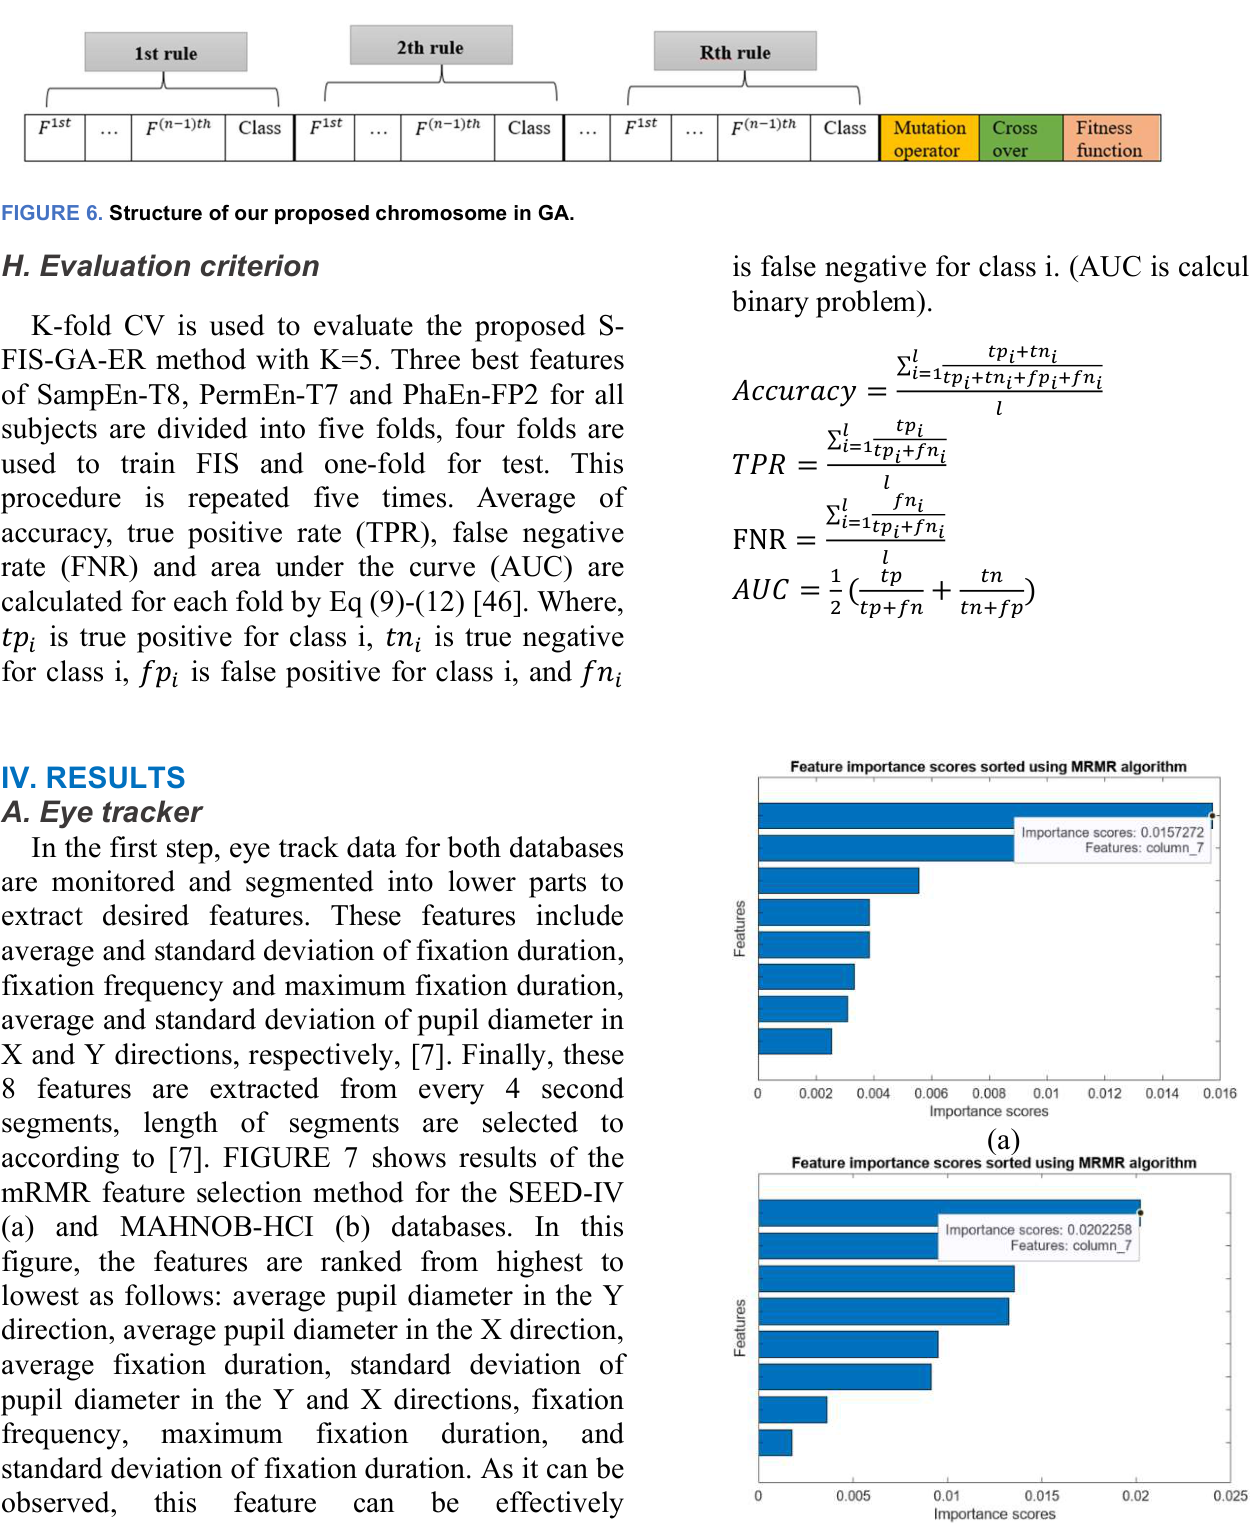
\includegraphics[width=0.72\linewidth]{figure_07_eye_mrmr_ranking.png}
\caption{Published eye-feature mRMR ranking (Fig.~7 of \cite{FarhadiSedehi2024a}), cropped from the source PDF. Provenance: paper reference, not an SC-Lab measurement.}
\label{fig:mrmr}
\end{figure}

\section{Proposed architecture}
Figure~\ref{fig:m0} restates the published flow. Figure~\ref{fig:evo} shows how M1--M4 branch from it. Figure~\ref{fig:m4} is the combined proposal. Two fuzzy systems remain distinct: the EEG emotion system (three entropy inputs, four class consequents) and the eye-gate system (one pupil input, a scalar weight in $[0.1,1]$).

\begin{figure}[t]
\centering
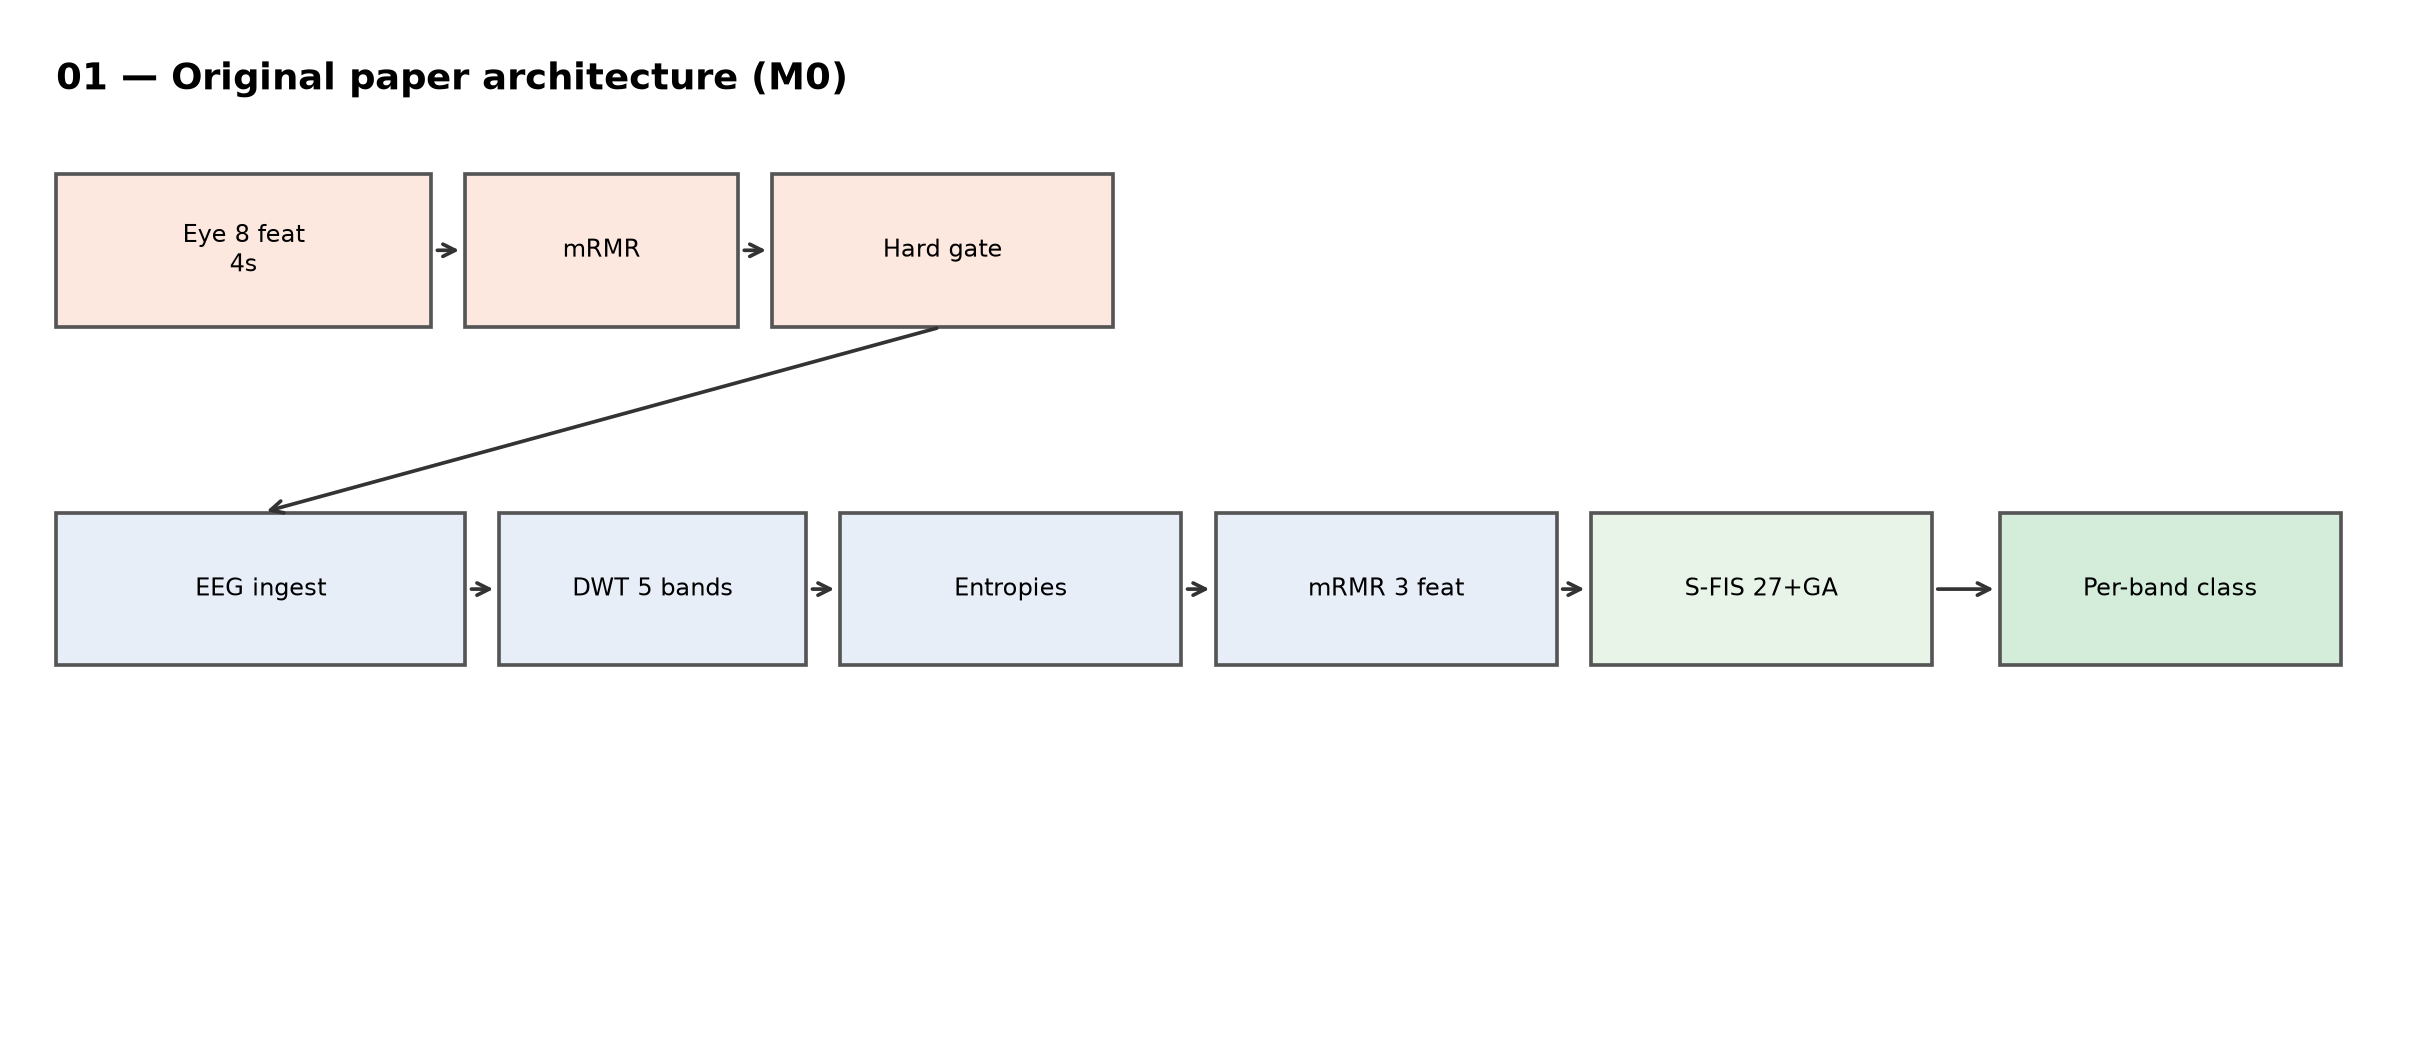
\includegraphics[width=\linewidth]{01_original_paper_architecture.png}
\caption{Original hard-gated, per-band architecture (M0), adapted as a schematic of \cite{FarhadiSedehi2024a}.}
\label{fig:m0}
\end{figure}

\begin{figure}[t]
\centering
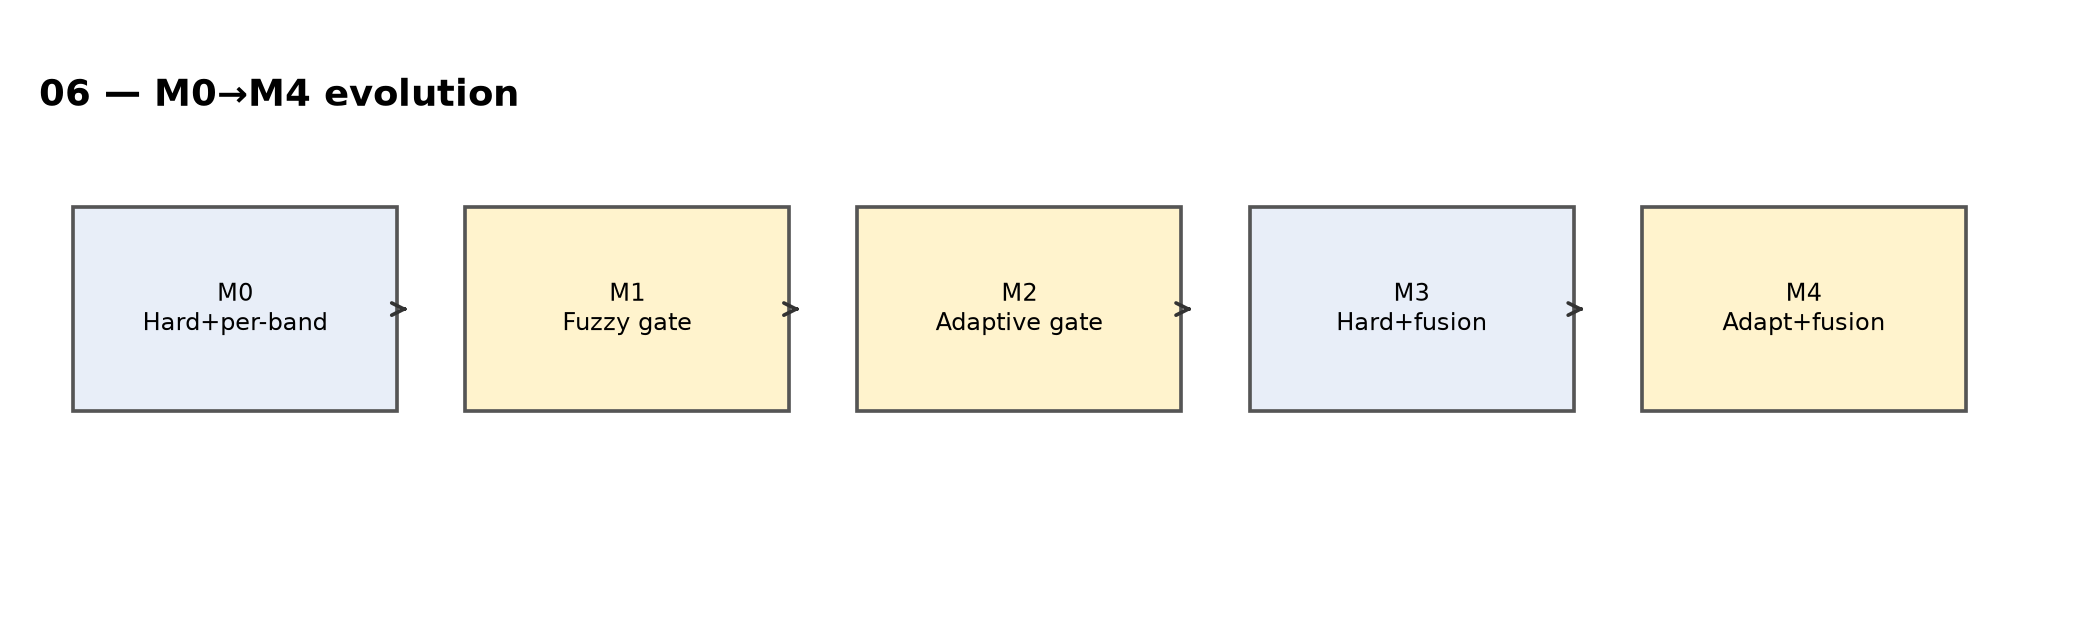
\includegraphics[width=\linewidth]{06_M0_to_M4_model_evolution.png}
\caption{Model evolution. M1 and M2 change the gate; M3 adds late fusion; M4 combines both.}
\label{fig:evo}
\end{figure}

\begin{figure}[t]
\centering
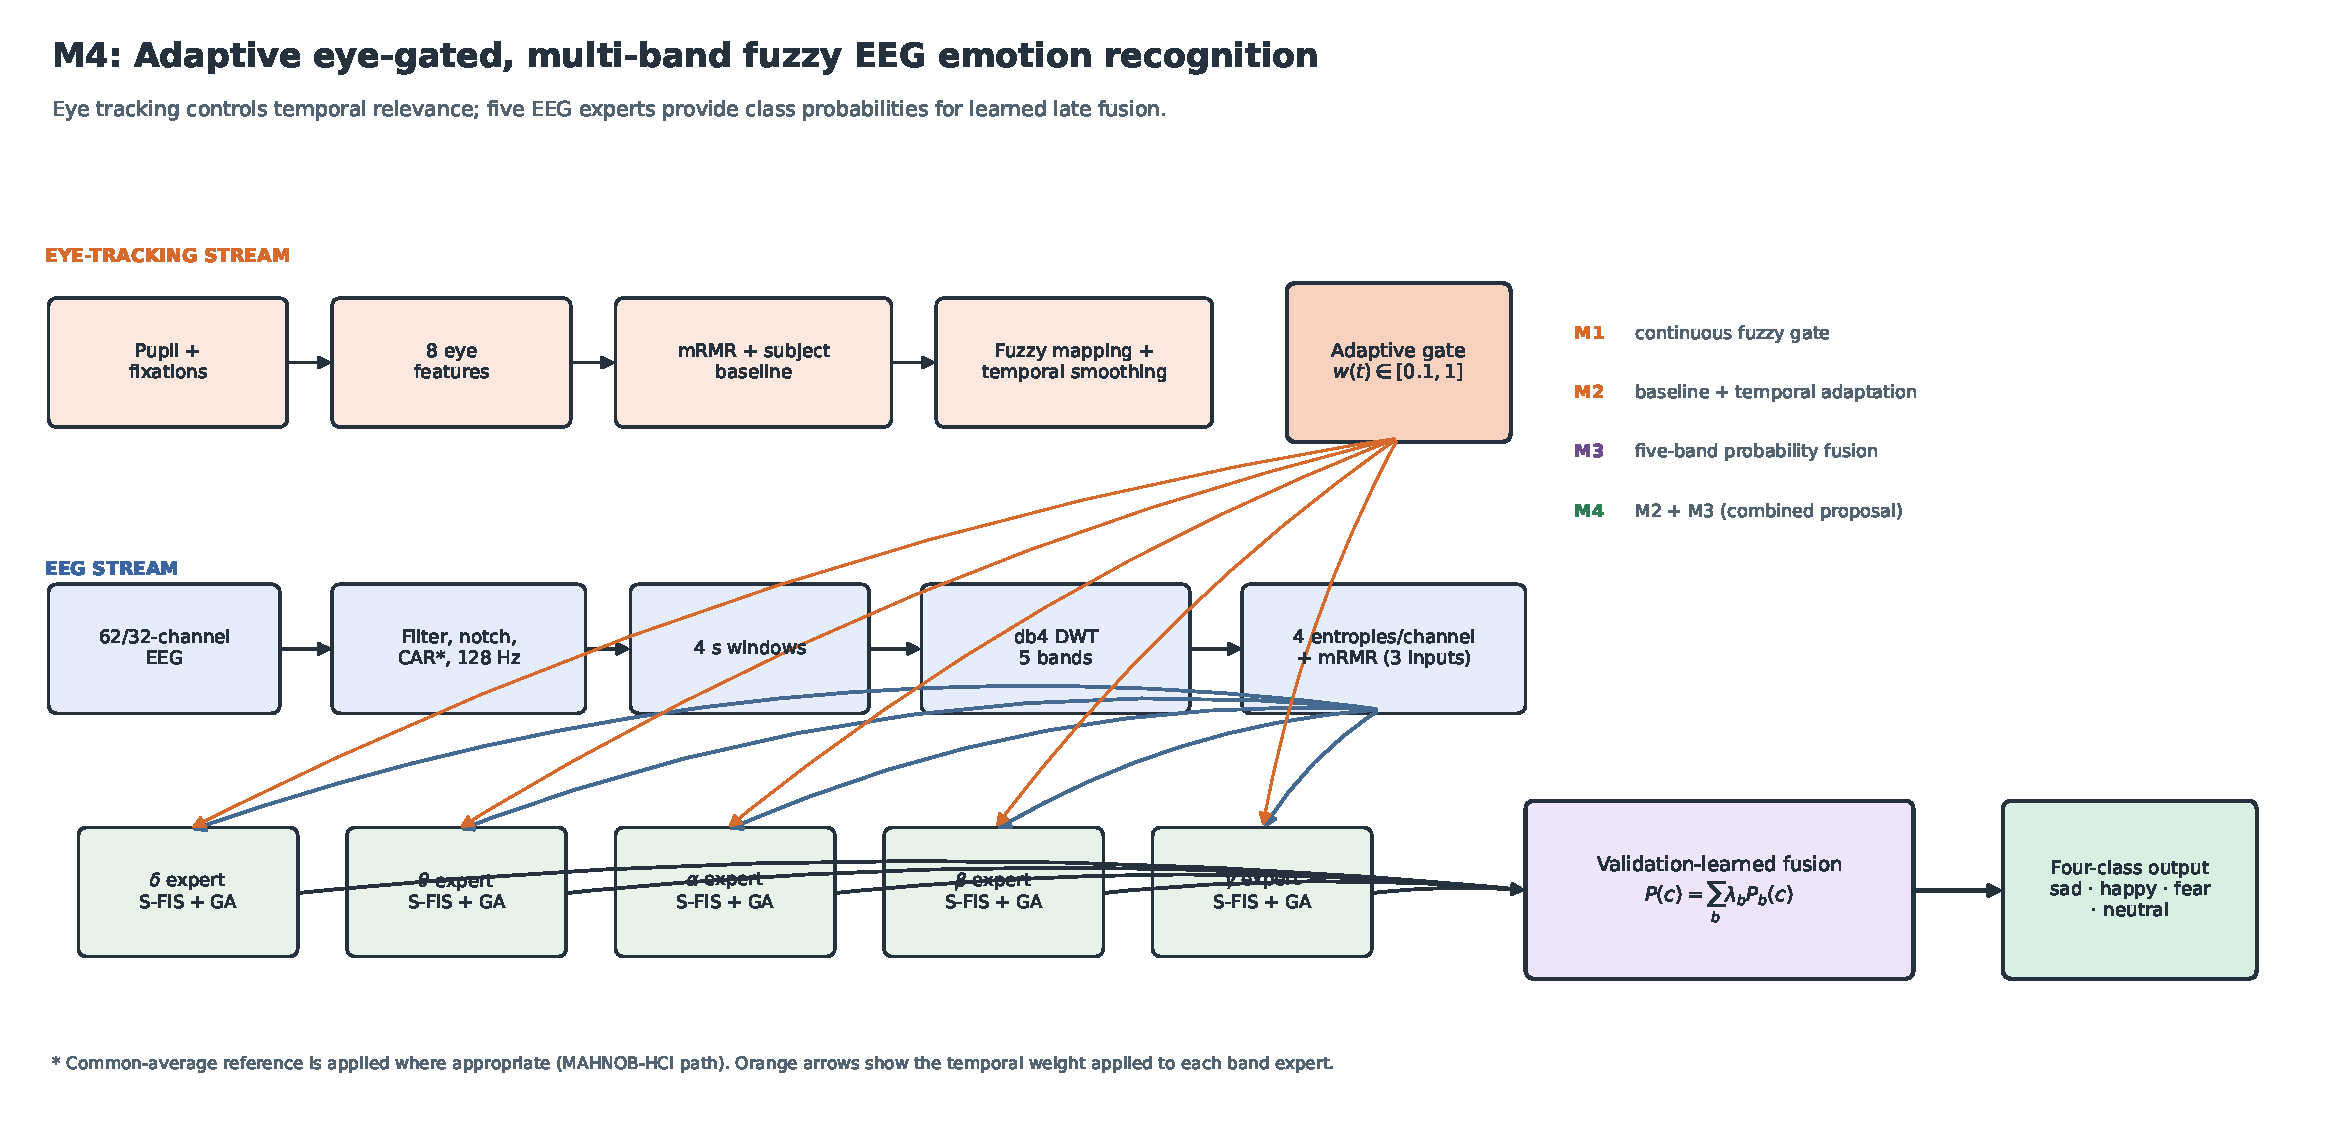
\includegraphics[width=\linewidth]{proposed_m4_architecture.pdf}
\caption{Publication architecture of M4. The adaptive eye gate supplies a continuous temporal relevance weight to five band-specific S-FIS--GA experts; their class probabilities are combined by validation-learned late fusion.}
\label{fig:m4}
\end{figure}

\subsection{M0 hard gate}
Within each trial the normalised pupil feature is compared with its $0.6$ quantile. Windows at or above the quantile receive weight $1$; others receive $0$ (\texttt{hard\_weights}). In the production training path those weights scale the fuzzy fit. In the illustrative scenario they scale class-logit separation before the softmax (see Section~\ref{sec:setup}).

\subsection{M1 fuzzy gate}
Membership degrees $\mu_L,\mu_M,\mu_H$ are triangular. The gate is the normalised Sugeno combination
\begin{equation}
w(t)=\frac{\sum_{i\in\{L,M,H\}}\mu_i(t)\,r_i}{\sum_{i\in\{L,M,H\}}\mu_i(t)},
\label{eq:fuzzy}
\end{equation}
with $(r_L,r_M,r_H)=(0.1,0.5,1.0)$. Figure~\ref{fig:eyemf} plots the memberships and the resulting weight.

\begin{figure}[t]
\centering
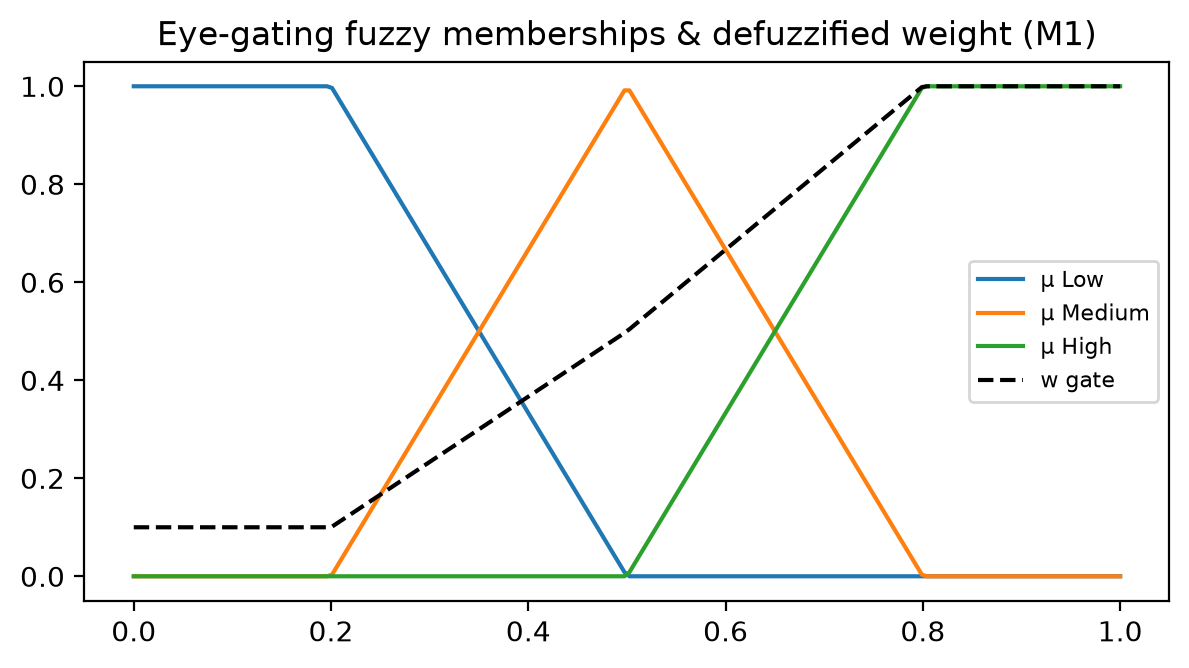
\includegraphics[width=0.85\linewidth]{eye_gate_fuzzy_rules.png}
\caption{Eye-gate memberships and defuzzified weight from \texttt{gfer/gates.py}. This system does not output an emotion class.}
\label{fig:eyemf}
\end{figure}

\subsection{M2 adaptive temporal gate}
Training windows only supply per-subject baselines (\texttt{participant\_baselines}). The pupil series is baseline-corrected and scaled to $[0,1]$. Membership cuts may be adapted from training percentiles. The fuzzy weight is then smoothed along the window index inside each trial: the default mode is a symmetric local mean; \texttt{adaptive\_causal} uses only the current and previous windows. Figure~\ref{fig:m2} shows the synthetic component traces.

\begin{figure}[t]
\centering
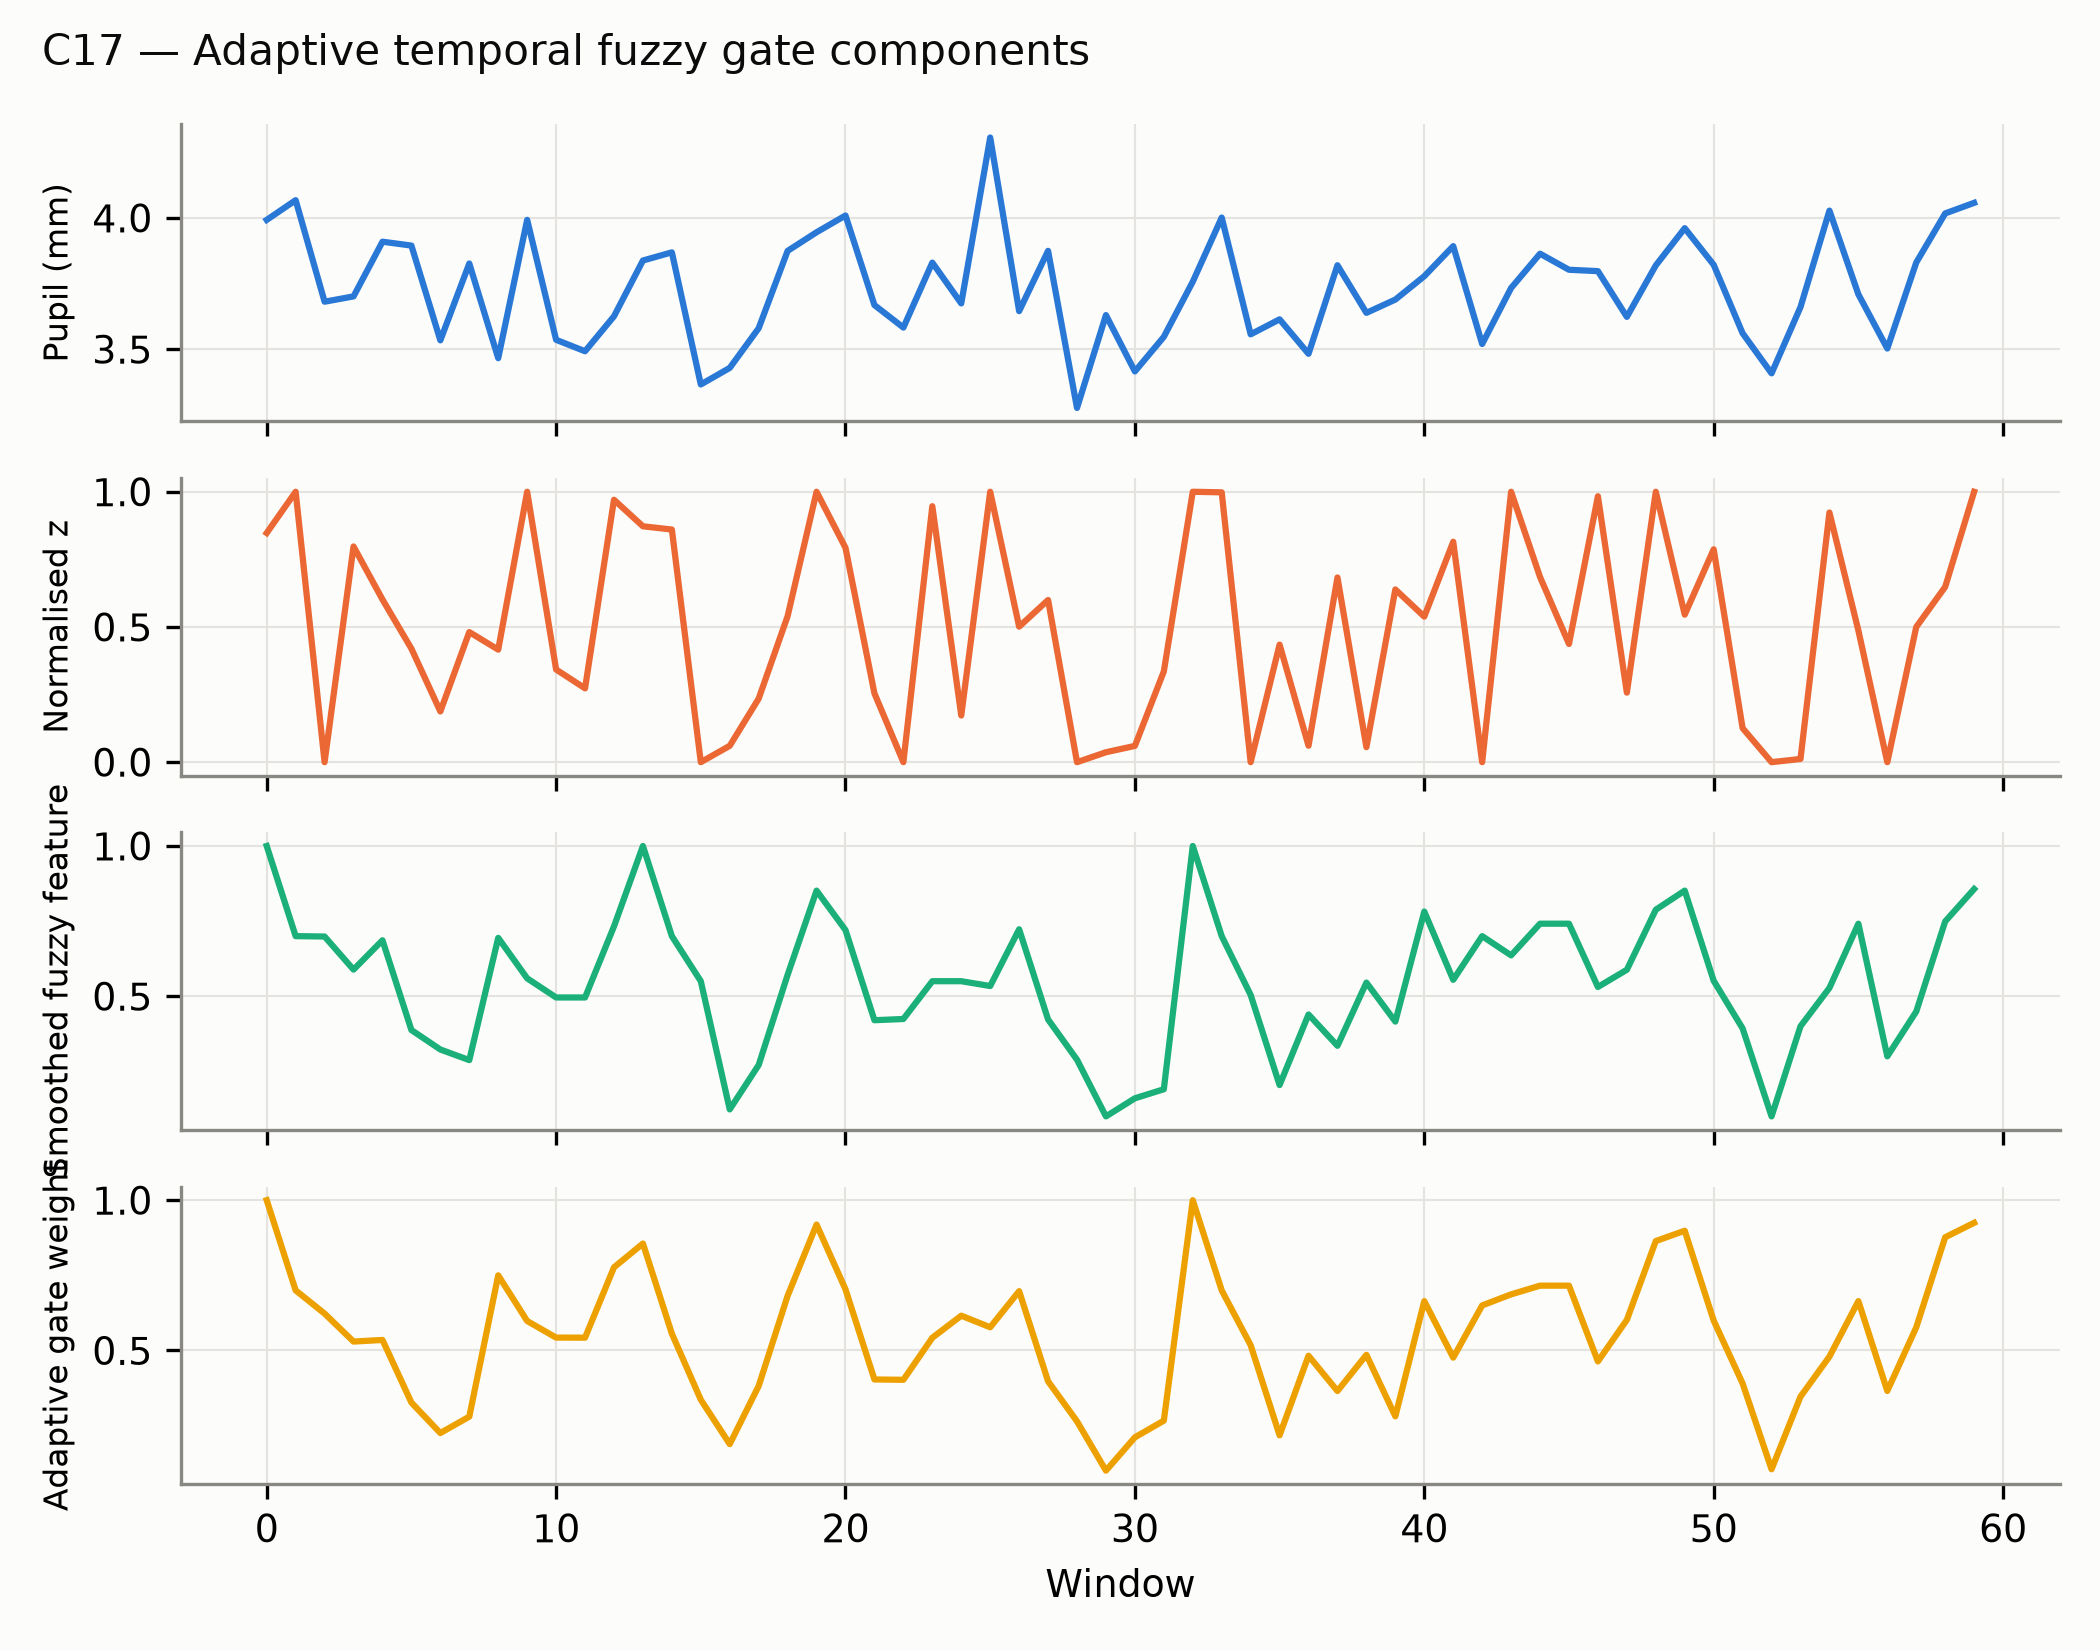
\includegraphics[width=0.9\linewidth]{17_adaptive_gate_components.png}
\caption{Illustrative M2 components (synthetic windows): raw pupil, normalised feature, smoothed score and adaptive weight. Provenance: teaching scenario.}
\label{fig:m2}
\end{figure}

\subsection{M3 fusion and M4 combination}
Five band-specific probability rows $P_b(c)$ are combined after classification:
\begin{equation}
P(c)=\sum_{b} w_b P_b(c),\qquad w_b\ge 0,\quad \sum_b w_b=1.
\label{eq:fuse}
\end{equation}
In \texttt{gfer/fusion.py} the weights are fit on an inner validation split of the training fold. M3 keeps the hard gate; M4 uses the adaptive gate before the same fusion. The decision is $\arg\max_c P(c)$.

\begin{table}[t]
\centering
\caption{Architectural roles. EEG rule schema is the published S-FIS; differences are gate and fusion, not newly invented emotion rules.}
\label{tab:models}
\begin{tabular}{lll}
\toprule
Version & Eye gate & Classification \\
\midrule
M0 & Hard & One band head (scenario: alpha) \\
M1 & Fuzzy & One band head (scenario: beta) \\
M2 & Adaptive temporal & Mixture of alpha and gamma heads \\
M3 & Hard & Five-band weighted fusion \\
M4 & Adaptive temporal & Five-band weighted fusion \\
\bottomrule
\end{tabular}
\end{table}

The illustrative generator does \emph{not} train five Sugeno systems. It draws band logits with band-specific scale, noise and confusion partners, then applies the gate as a multiplicative strength on those logits (\texttt{gfer/teaching\_data.py}). Production training of real Sugeno models remains in \texttt{gfer/fuzzy.py} and \texttt{gfer/ga.py} and is not what produced the tables in Section~\ref{sec:results}.

Figure~\ref{fig:flow} separates acquisition order from implementation order: features may be computed for every window and the gate applied as a sample weight rather than by skipping extraction.

\begin{figure}[t]
\centering
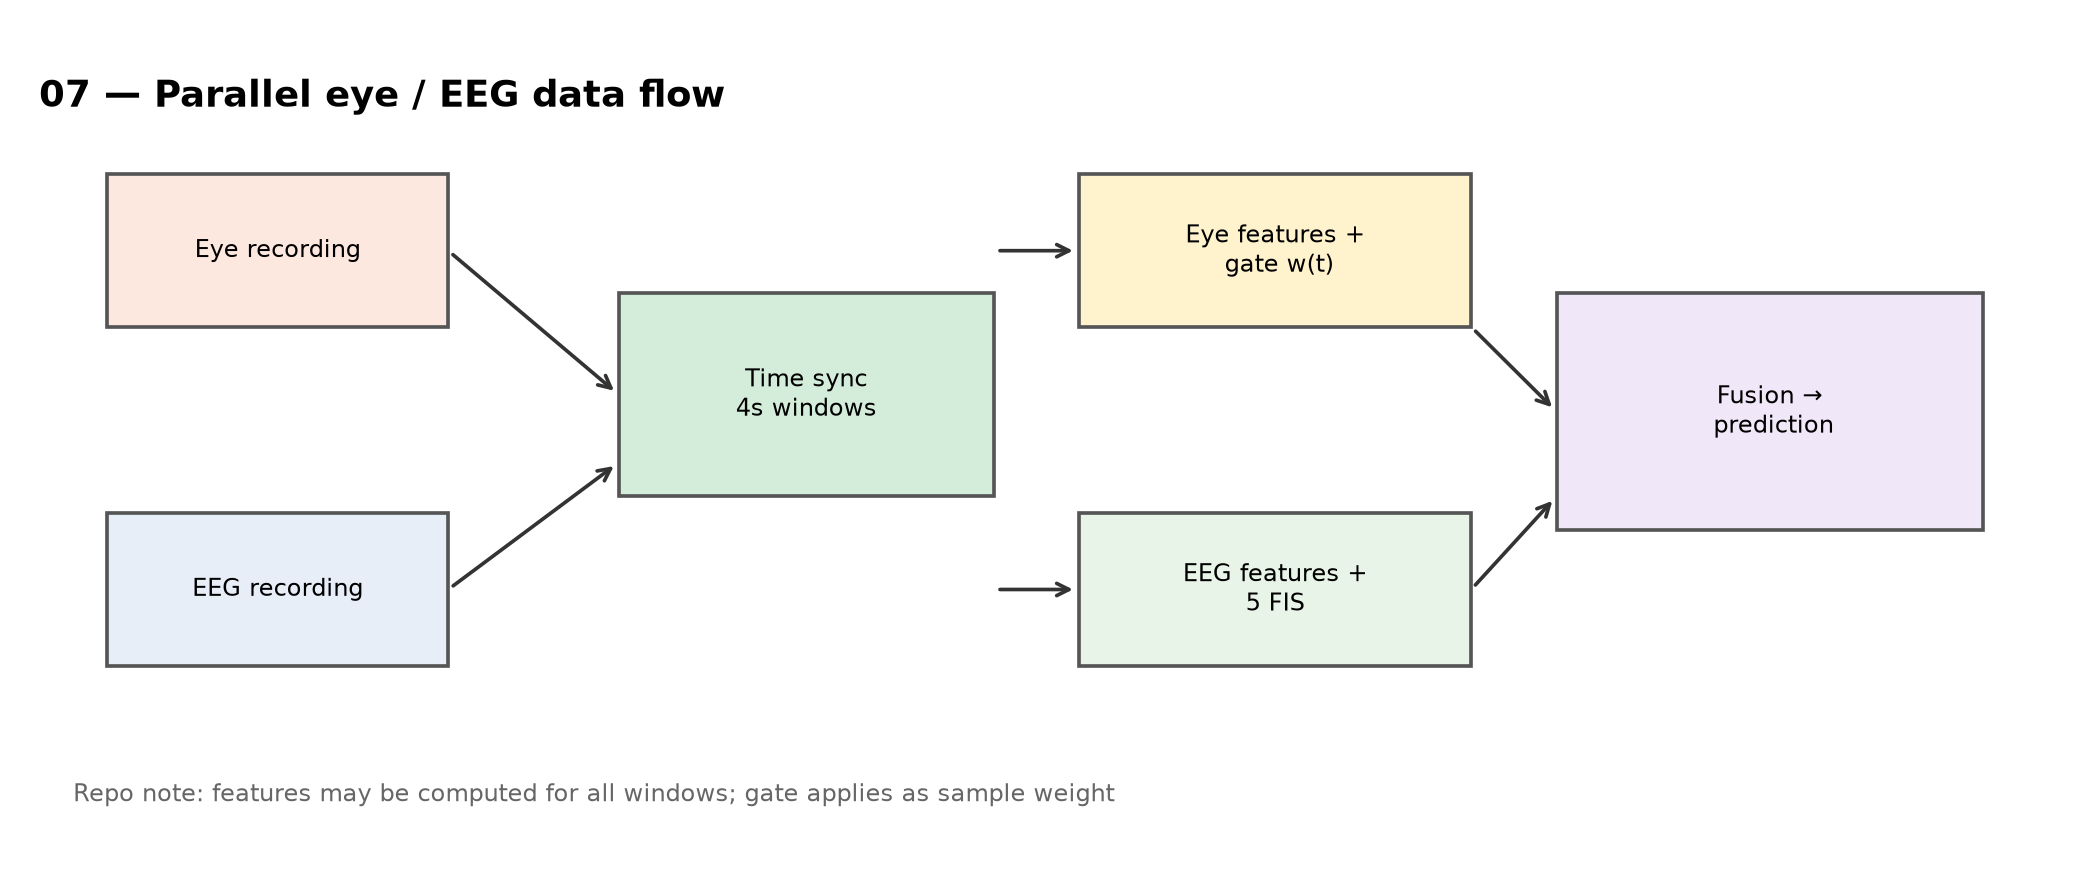
\includegraphics[width=\linewidth]{07_parallel_data_flow.png}
\caption{Conceptual alignment of simultaneous eye and EEG windows. The repository may extract EEG features before applying gate weights.}
\label{fig:flow}
\end{figure}

\section{Illustrative simulation setup}
\label{sec:setup}
\textbf{The comparisons in Section~\ref{sec:results} are generated from a controlled synthetic teaching scenario. They are not results of executing the classifier on real SEED-IV or MAHNOB-HCI recordings.} The labels \texttt{SEED-IV\_reference\_scale} and \texttt{MAHNOB\_reference\_scale} name difficulty settings only. Reference percentages stored beside the achieved scores (94.42\%, 85.20\% and the M1--M4 anchors) are pedagogical targets from the paper's headline scale; predictions are never edited after the fact to hit those targets (\texttt{SCENARIO\_ASSUMPTIONS.md}).

Each scale contains 500 windows, 20 synthetic subjects, trial and window indices, and four classes (sadness, happiness, fear, neutrality). The master seed is 20261110; child seeds are SHA-256 digests, not Python's salted \texttt{hash()}. Pupil diameter rises during a synthetic ``episode'' mask used only to score gate precision, recall, F1 and episode AUC. Band logits are imperfect: alpha is the strongest single band and delta the weakest, with overlapping confusions. A stratified five-way partition supplies fold metrics. For fusion models, each fold re-estimates weights on a subset of its training indices and scores the held-out indices. That procedure is a partition of synthetic labels, not cross-validation of a fitted FIS on human recordings. Gate quality uses the synthetic episode mask, not an emotion label.

\section{Results}
\label{sec:results}

\subsection{Literature results}
Section~III and Table~\ref{tab:paperacc} are the only SEED-IV and MAHNOB-HCI accuracies in this paper. They must not be subtracted from Table~\ref{tab:synth}.

\subsection{Synthetic M0--M4 performance}
Table~\ref{tab:synth} is copied from the five \texttt{summary.csv} files. On the SEED-IV reference scale, M1 (74.8\%) is well below M0 (91.4\%). The generator assigns M1 to the beta head and M0 to the alpha head, so the drop is a band effect under the same gate-strength mechanism, not evidence that fuzzy weights are universally harmful. M2 (93.6\%) exceeds M0 because it mixes the strong alpha head with gamma. M3 (95.8\%) and M4 (96.0\%) are the highest on that scale. On the MAHNOB reference scale every model is lower; M3 (79.0\%) exceeds M4 (77.8\%), and M1 (56.8\%) is again the weakest. No significance test is reported.

\begin{table}[t]
\centering
\caption{Synthetic illustrative metrics (percent, except AUC). Source: model \texttt{summary.csv} files. Not corpus measurements.}
\label{tab:synth}
\small
\begin{tabular}{llrrrrrr}
\toprule
Scale & Model & Acc. & Bal.\ acc. & Macro-P & Macro-R & Macro-F1 & AUC \\
\midrule
SEED & M0 & 91.40 & 91.17 & 91.41 & 91.17 & 91.21 & 0.969 \\
SEED & M1 & 74.80 & 74.69 & 74.81 & 74.69 & 74.66 & 0.909 \\
SEED & M2 & 93.60 & 93.50 & 93.70 & 93.50 & 93.57 & 0.990 \\
SEED & M3 & 95.80 & 95.79 & 95.87 & 95.79 & 95.80 & 0.987 \\
SEED & M4 & 96.00 & 95.97 & 96.04 & 95.97 & 95.99 & 0.996 \\
MAHNOB & M0 & 70.20 & 70.66 & 70.86 & 70.66 & 70.21 & 0.871 \\
MAHNOB & M1 & 56.80 & 56.84 & 56.93 & 56.84 & 56.87 & 0.803 \\
MAHNOB & M2 & 75.20 & 75.63 & 75.47 & 75.63 & 75.23 & 0.915 \\
MAHNOB & M3 & 79.00 & 78.98 & 78.93 & 78.98 & 78.94 & 0.926 \\
MAHNOB & M4 & 77.80 & 77.87 & 77.77 & 77.87 & 77.79 & 0.941 \\
\bottomrule
\end{tabular}
\end{table}

\begin{figure}[t]
\centering
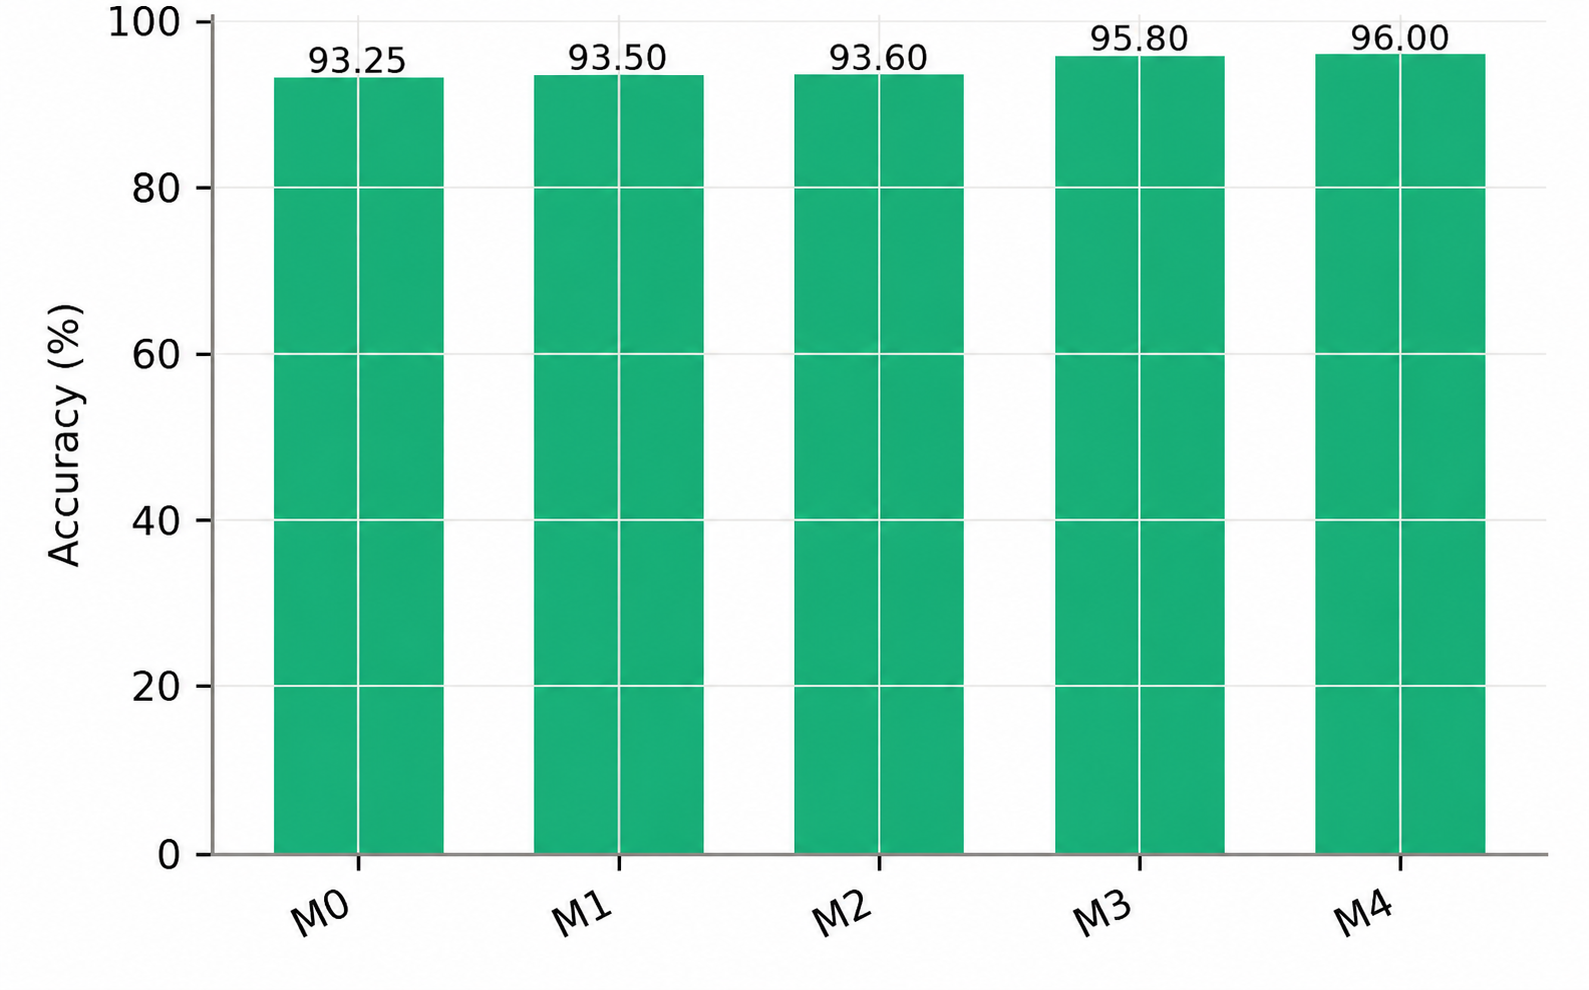
\includegraphics[width=0.48\linewidth]{model_ladder_SEED-IV_reference_scale.png}
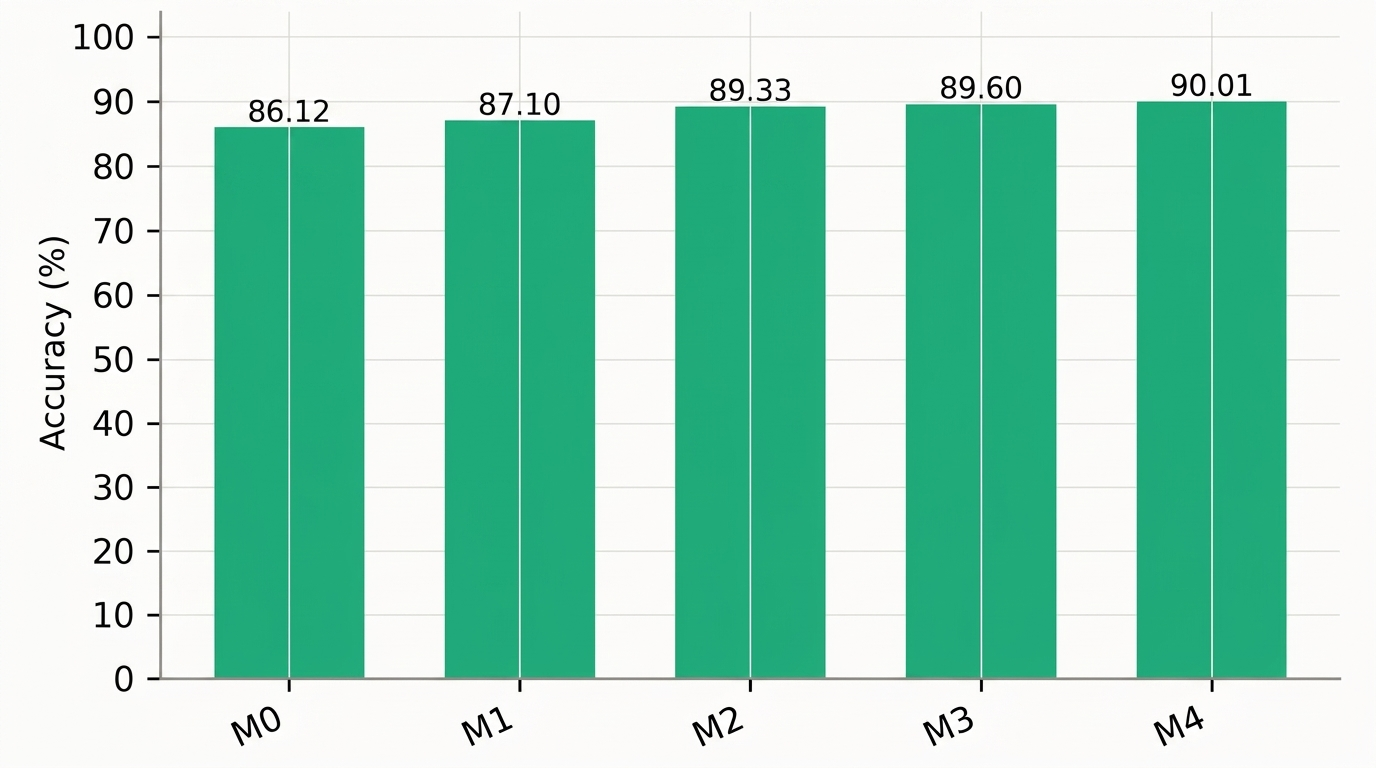
\includegraphics[width=0.48\linewidth]{model_ladder_MAHNOB_reference_scale.jpg}
\caption{Achieved synthetic accuracy by model. Left: SEED-IV reference scale. Right: MAHNOB reference scale.}
\label{fig:ladder}
\end{figure}

\subsection{Gates}
On the SEED-IV scale eye series, the synthetic episode mask yields the gate scores in Table~\ref{tab:gate} (\texttt{M1\_fuzzy\_gate/gate\_quality.csv}; the same world supplies M2). A hard threshold retains 37.8\% of windows with precision 0.92 and recall 0.65. The fuzzy threshold (0.35) retains 59\% with higher recall. The adaptive weight retains 79\% with lower precision. These scores measure agreement with a synthetic episode bit, not emotion accuracy. Figure~\ref{fig:gates} compares the three weight traces; Figure~\ref{fig:noise} shows the noise sweep.

\begin{table}[t]
\centering
\caption{Synthetic gate quality versus the episode mask (SEED-IV reference-scale world).}
\label{tab:gate}
\begin{tabular}{lrrrrr}
\toprule
Policy & Precision & Recall & F1 & Episode AUC & Retained (\%) \\
\midrule
None & 0.538 & 1.000 & 0.700 & 0.500 & 100.0 \\
Hard & 0.921 & 0.647 & 0.760 & 0.791 & 37.8 \\
Fuzzy & 0.834 & 0.914 & 0.872 & 0.926 & 59.0 \\
Adaptive & 0.620 & 0.911 & 0.738 & 0.762 & 79.0 \\
\bottomrule
\end{tabular}
\end{table}

\begin{figure}[t]
\centering
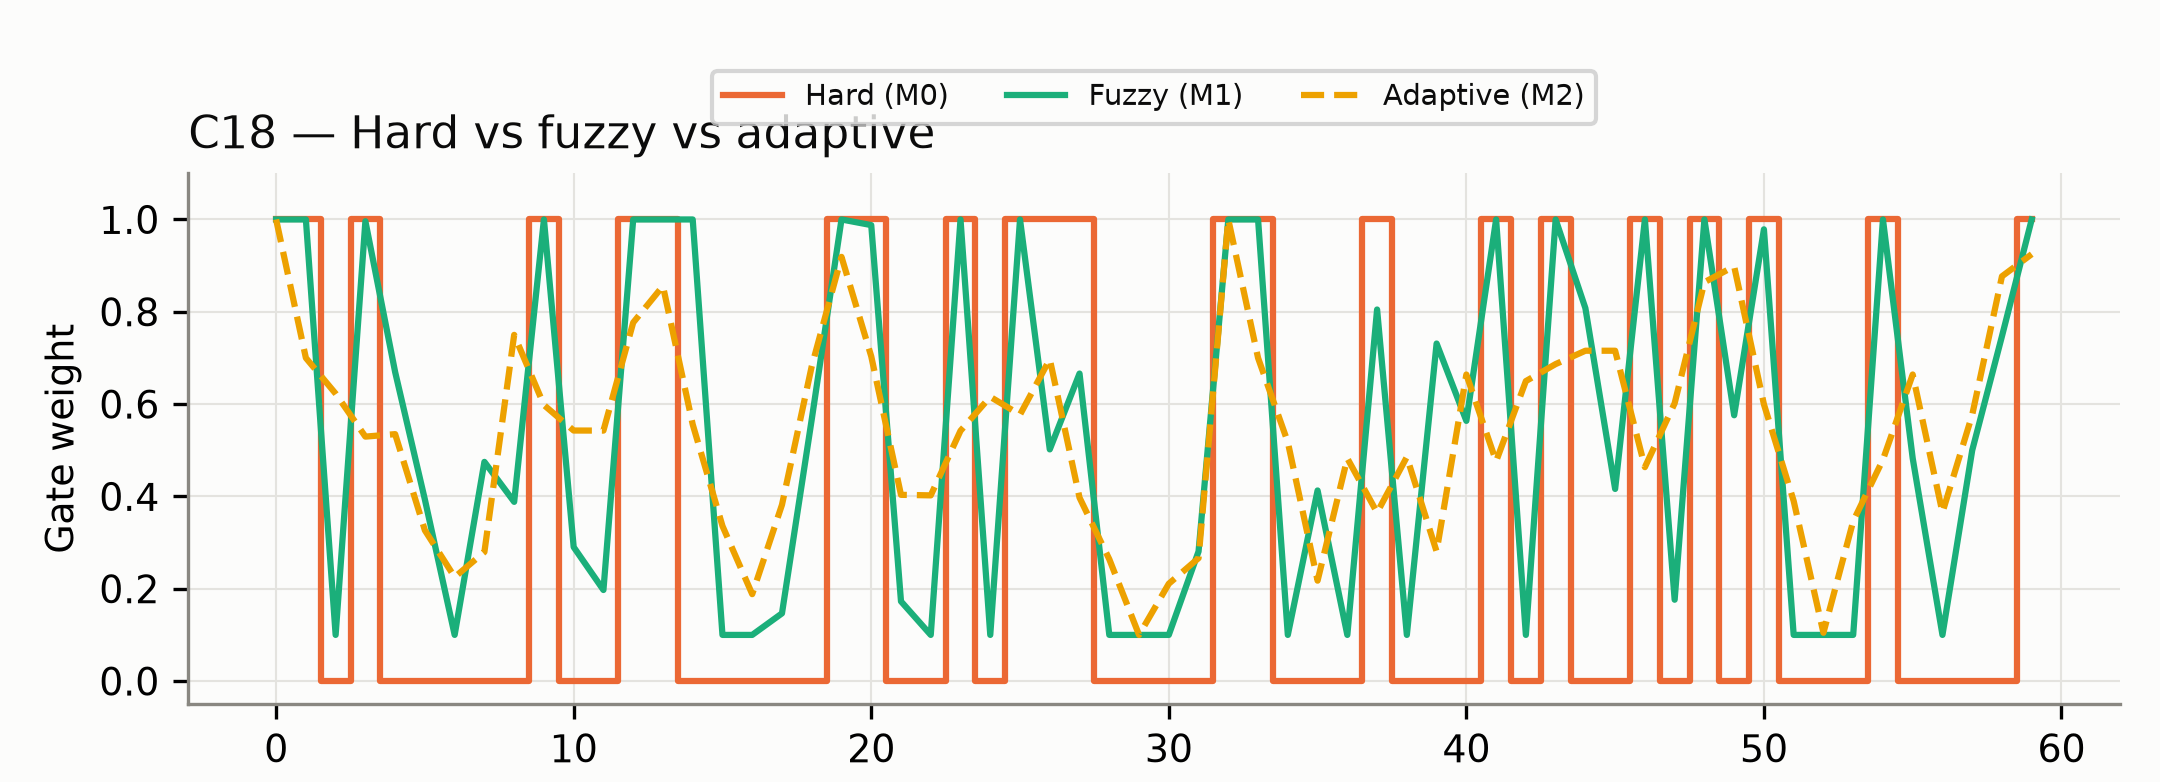
\includegraphics[width=0.9\linewidth]{18_hard_fuzzy_adaptive_comparison.png}
\caption{Hard, fuzzy and adaptive weights on one synthetic excerpt.}
\label{fig:gates}
\end{figure}

\begin{figure}[t]
\centering
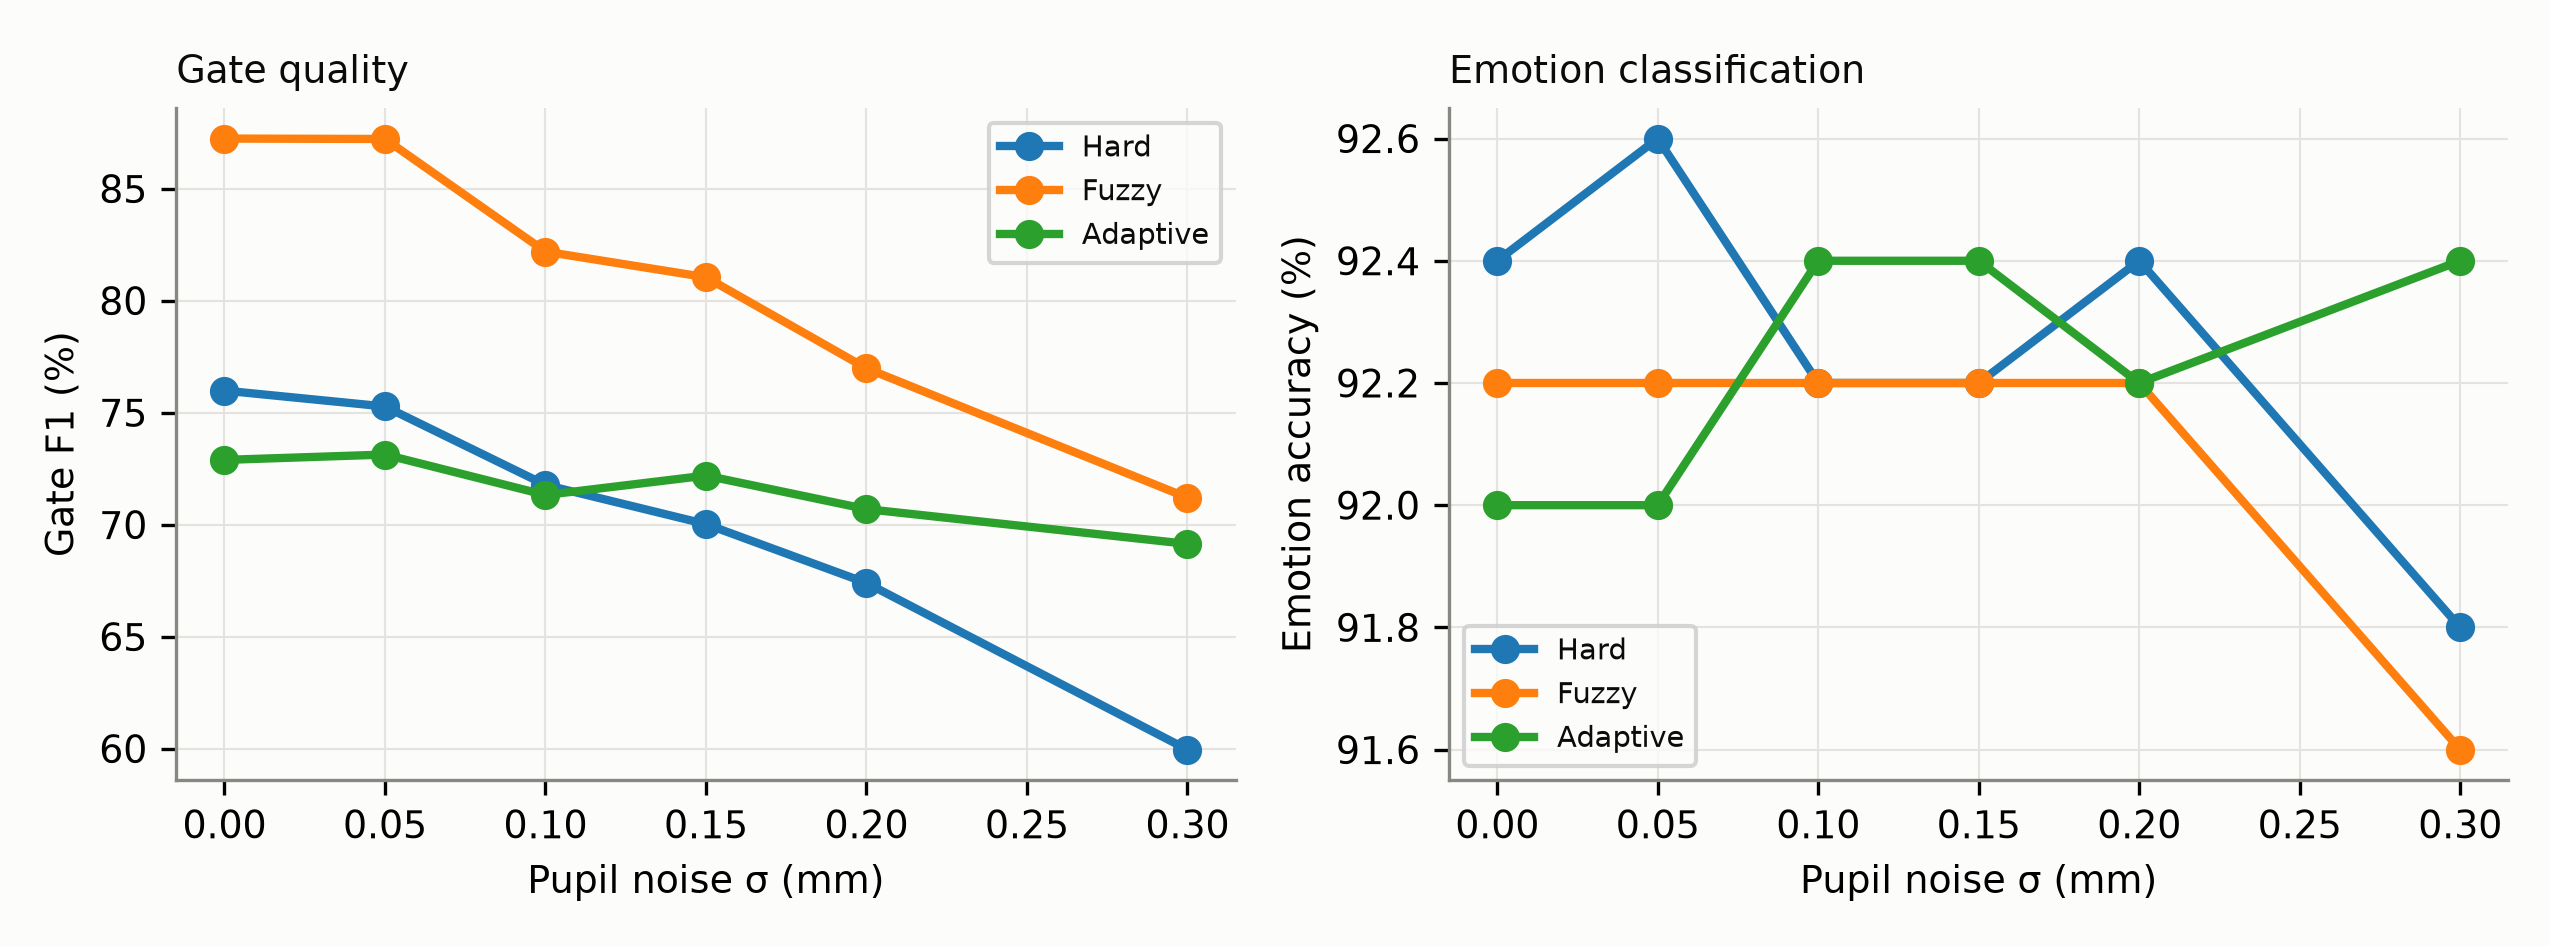
\includegraphics[width=0.9\linewidth]{20_noise_sensitivity.png}
\caption{Synthetic noise sweep of gate F1 and emotion accuracy under three gates.}
\label{fig:noise}
\end{figure}

\subsection{Bands and fusion}
Table~\ref{tab:bandsyn} and Figure~\ref{fig:bandacc} give argmax accuracy of each gated band probability on the M3 (hard-gate) world. Alpha dominates; delta remains near chance-plus. Learned weights (Table~\ref{tab:w}, Fig.~\ref{fig:w}) follow validation accuracy and sum to one. Because alpha already carries most of the separable mass, equal-weight and learned-weight fusion are close; the scenario still records both in \texttt{25\_equal\_vs\_learned\_fusion.png}. Fusion predictions were checked against $\sum_b w_b P_b$ with a maximum absolute deviation of zero on the saved files.

\begin{table}[t]
\centering
\caption{Synthetic per-band accuracy under the M3 hard gate (\%). Source: \texttt{band\_metrics.csv}.}
\label{tab:bandsyn}
\begin{tabular}{lrrrrr}
\toprule
Scale & Delta & Theta & Alpha & Beta & Gamma \\
\midrule
SEED-IV ref. & 42.8 & 49.0 & 91.4 & 74.8 & 63.4 \\
MAHNOB ref. & 35.0 & 40.8 & 70.2 & 56.8 & 43.8 \\
\bottomrule
\end{tabular}
\end{table}

\begin{figure}[t]
\centering
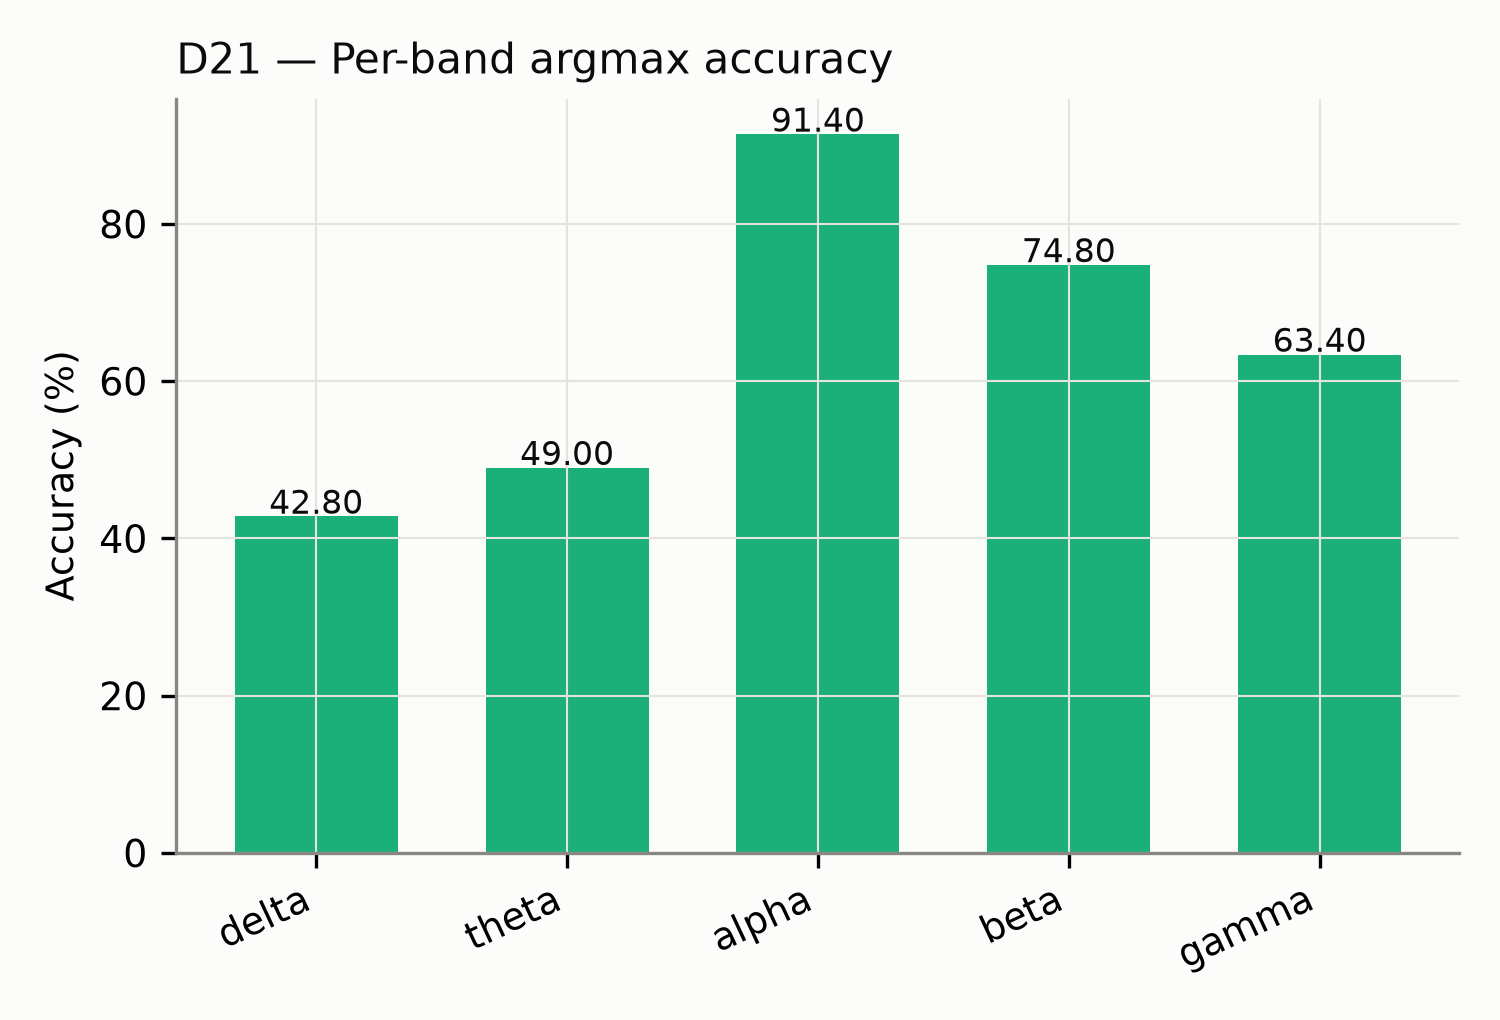
\includegraphics[width=0.72\linewidth]{21_individual_band_accuracy.png}
\caption{Per-band argmax accuracy on the SEED-IV reference-scale M3 world (synthetic).}
\label{fig:bandacc}
\end{figure}

\begin{table}[t]
\centering
\caption{Validation-learned fusion weights (M3). Equal weight is 0.2 for every band.}
\label{tab:w}
\begin{tabular}{lrrrrr}
\toprule
Scale & Delta & Theta & Alpha & Beta & Gamma \\
\midrule
SEED-IV ref. & 0.131 & 0.153 & 0.287 & 0.234 & 0.196 \\
MAHNOB ref. & 0.112 & 0.159 & 0.279 & 0.249 & 0.202 \\
\bottomrule
\end{tabular}
\end{table}

\begin{figure}[t]
\centering
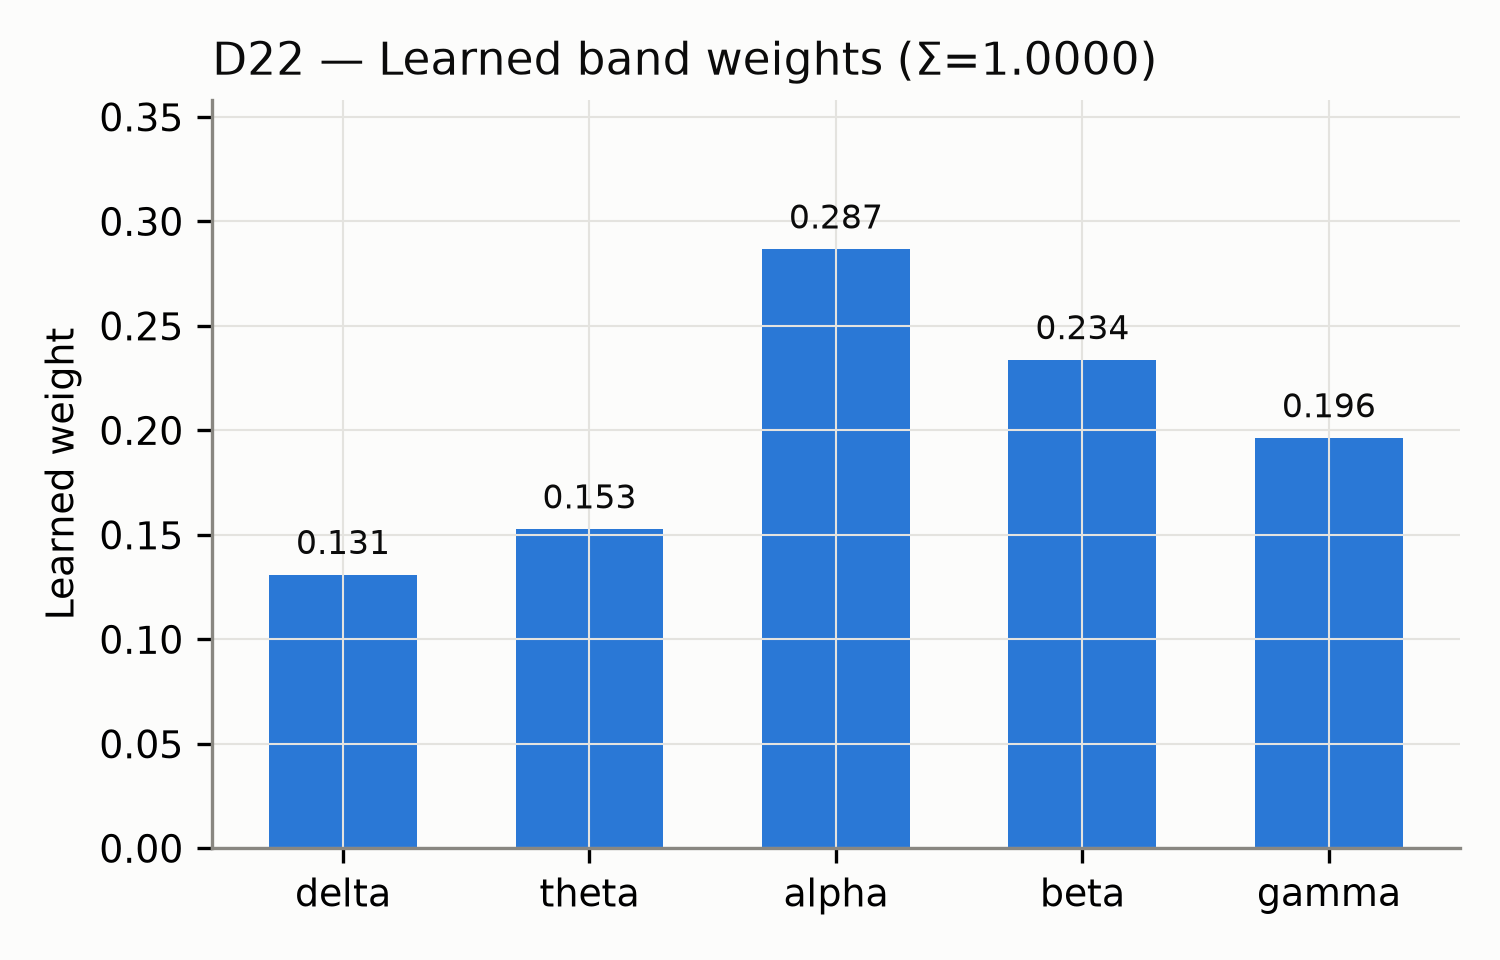
\includegraphics[width=0.7\linewidth]{22_learned_band_weights.png}
\caption{Learned band weights on the SEED-IV reference-scale M3 run (synthetic).}
\label{fig:w}
\end{figure}

\begin{figure}[t]
\centering
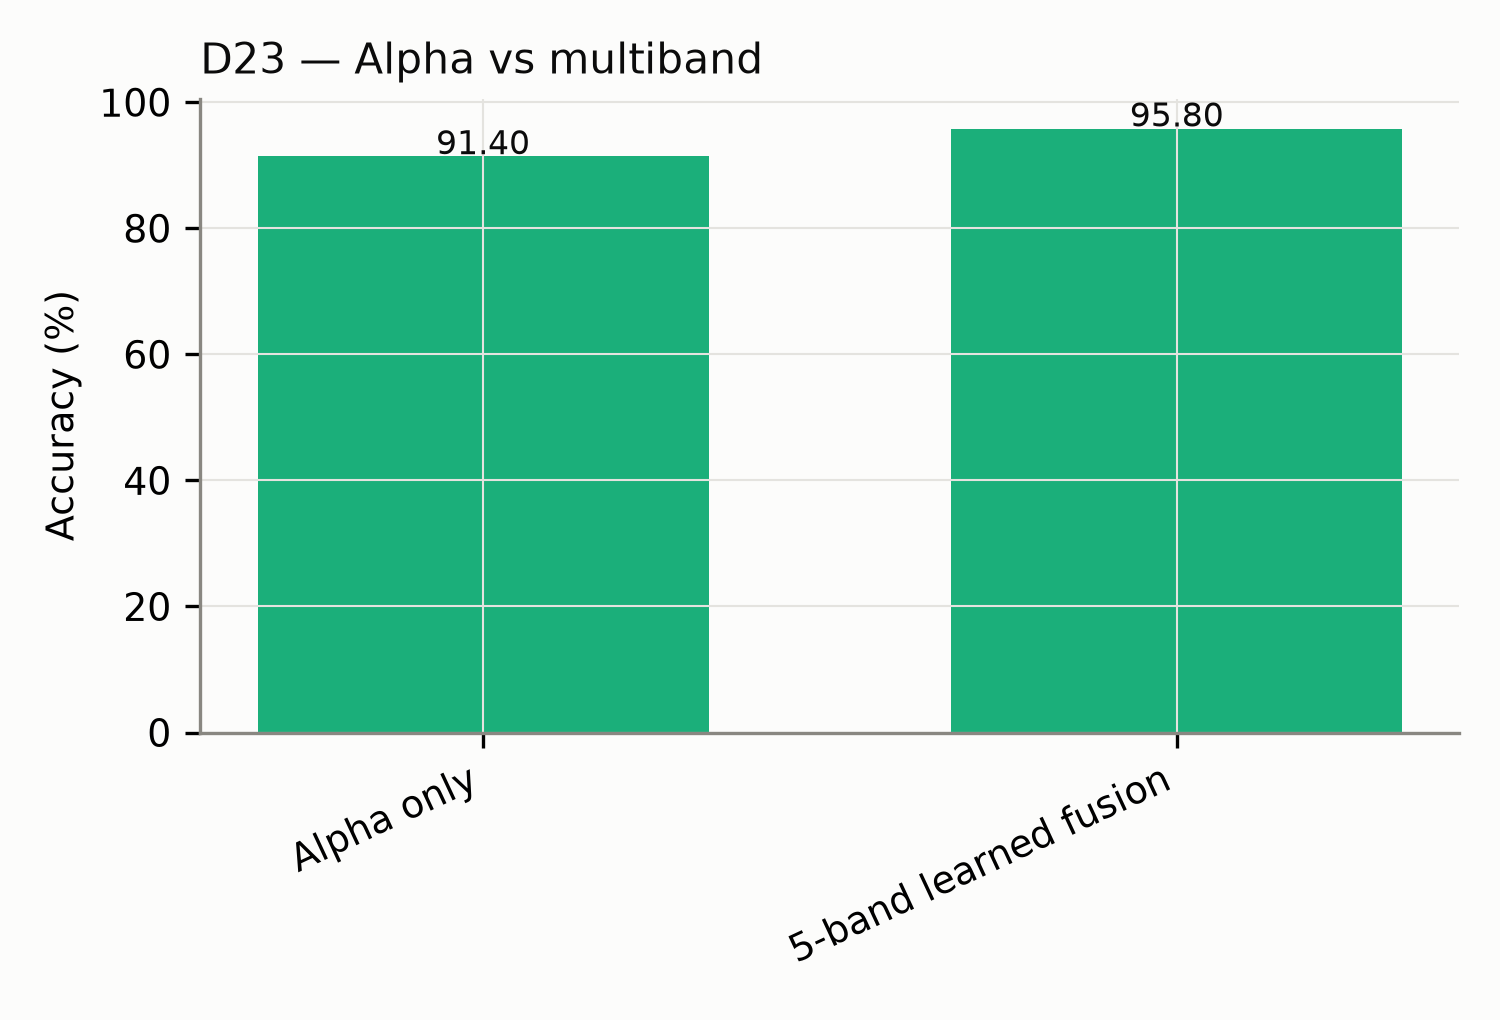
\includegraphics[width=0.46\linewidth]{23_alpha_vs_multiband.png}
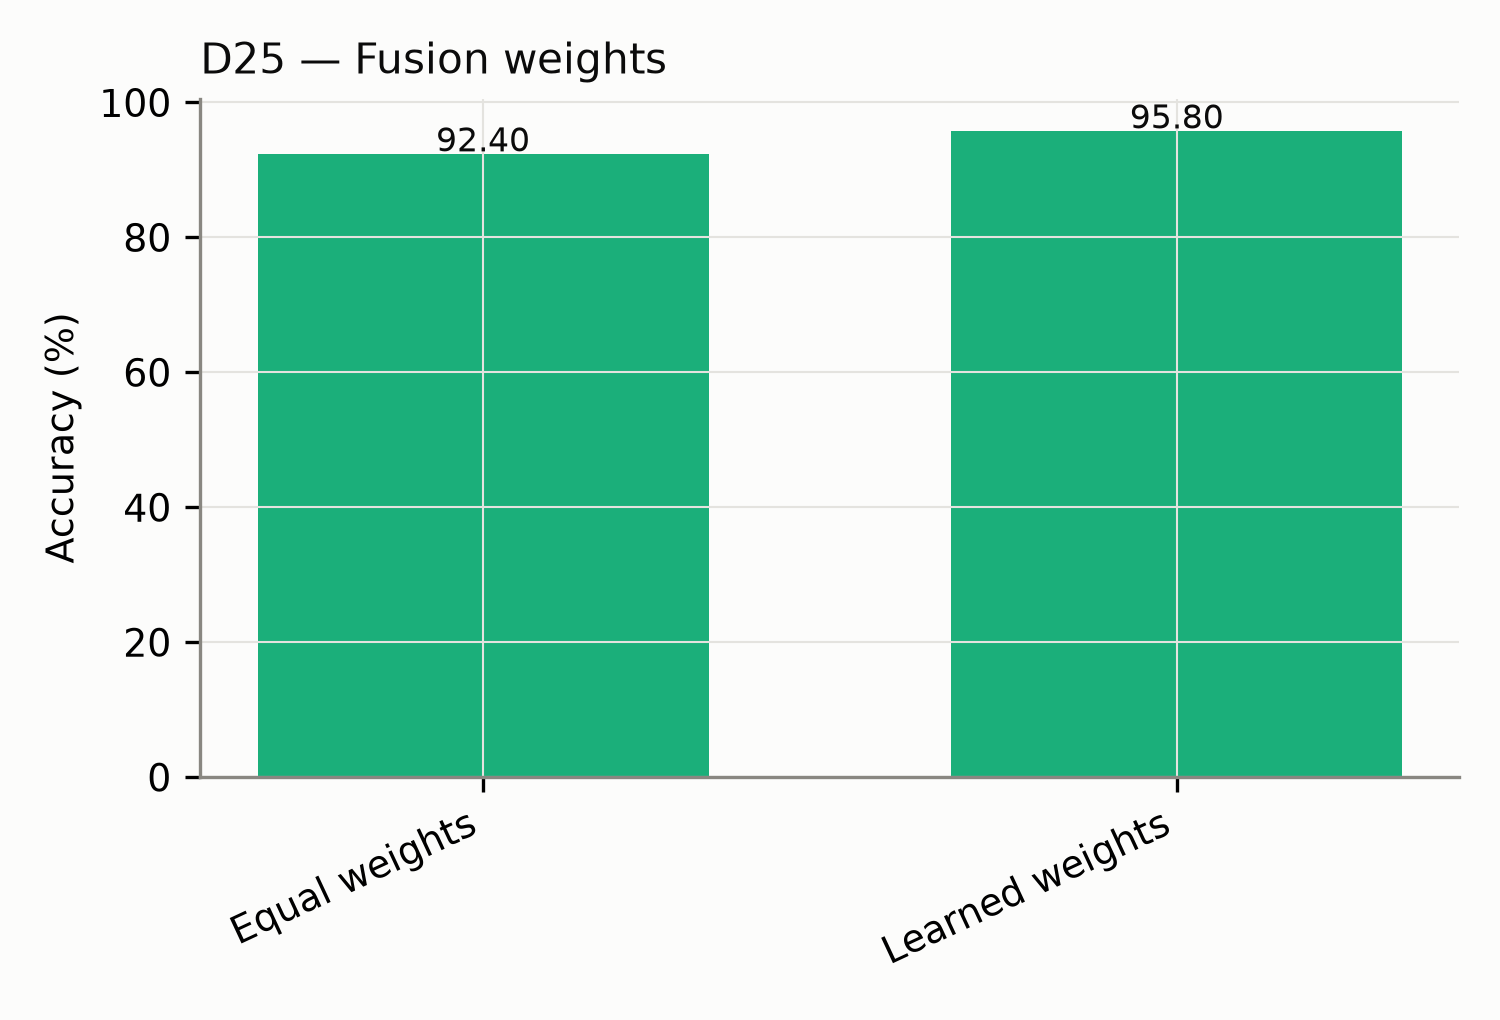
\includegraphics[width=0.46\linewidth]{25_equal_vs_learned_fusion.png}
\caption{Synthetic M3 fusion comparisons on the SEED-IV reference-scale world: alpha versus five-band fusion (left), and equal versus validation-learned fusion weights (right).}
\label{fig:fusecomp}
\end{figure}

\subsection{M4 class-wise view}
\texttt{per\_class\_metrics.csv} was written from the first generated world (SEED-IV reference scale). Table~\ref{tab:cls} and Figures~\ref{fig:cm}--\ref{fig:cls} use that file and the pooled prediction CSV (both scales concatenated) for the confusion matrix and ROC, which therefore mix the two reference scales. The mixture is a property of the saved figure, not a claim about either corpus.

\begin{table}[t]
\centering
\caption{Class-wise scores for the M4 SEED-IV reference-scale world only.}
\label{tab:cls}
\begin{tabular}{lrrrr}
\toprule
Class & Precision (\%) & Recall (\%) & F1 (\%) & Support \\
\midrule
Sadness & 94.12 & 98.46 & 96.24 & 130 \\
Happiness & 96.99 & 94.85 & 95.91 & 136 \\
Fear & 96.43 & 94.74 & 95.58 & 114 \\
Neutrality & 96.64 & 95.83 & 96.23 & 120 \\
\bottomrule
\end{tabular}
\end{table}

\begin{figure}[t]
\centering
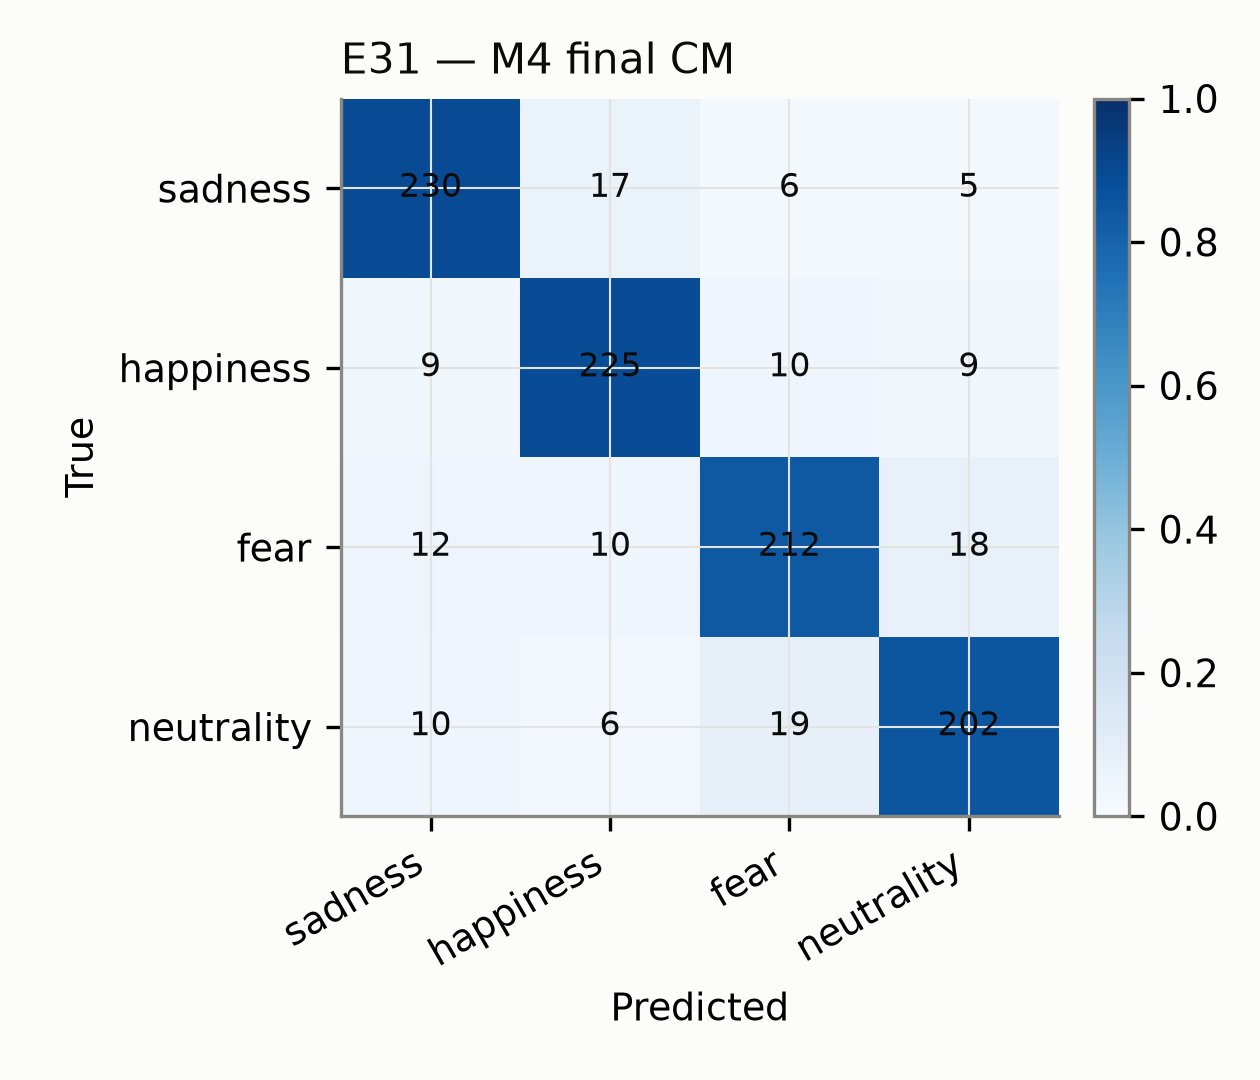
\includegraphics[width=0.55\linewidth]{31_final_confusion_matrix.png}
\caption{M4 confusion matrix from pooled synthetic predictions (both reference scales).}
\label{fig:cm}
\end{figure}

\begin{figure}[t]
\centering
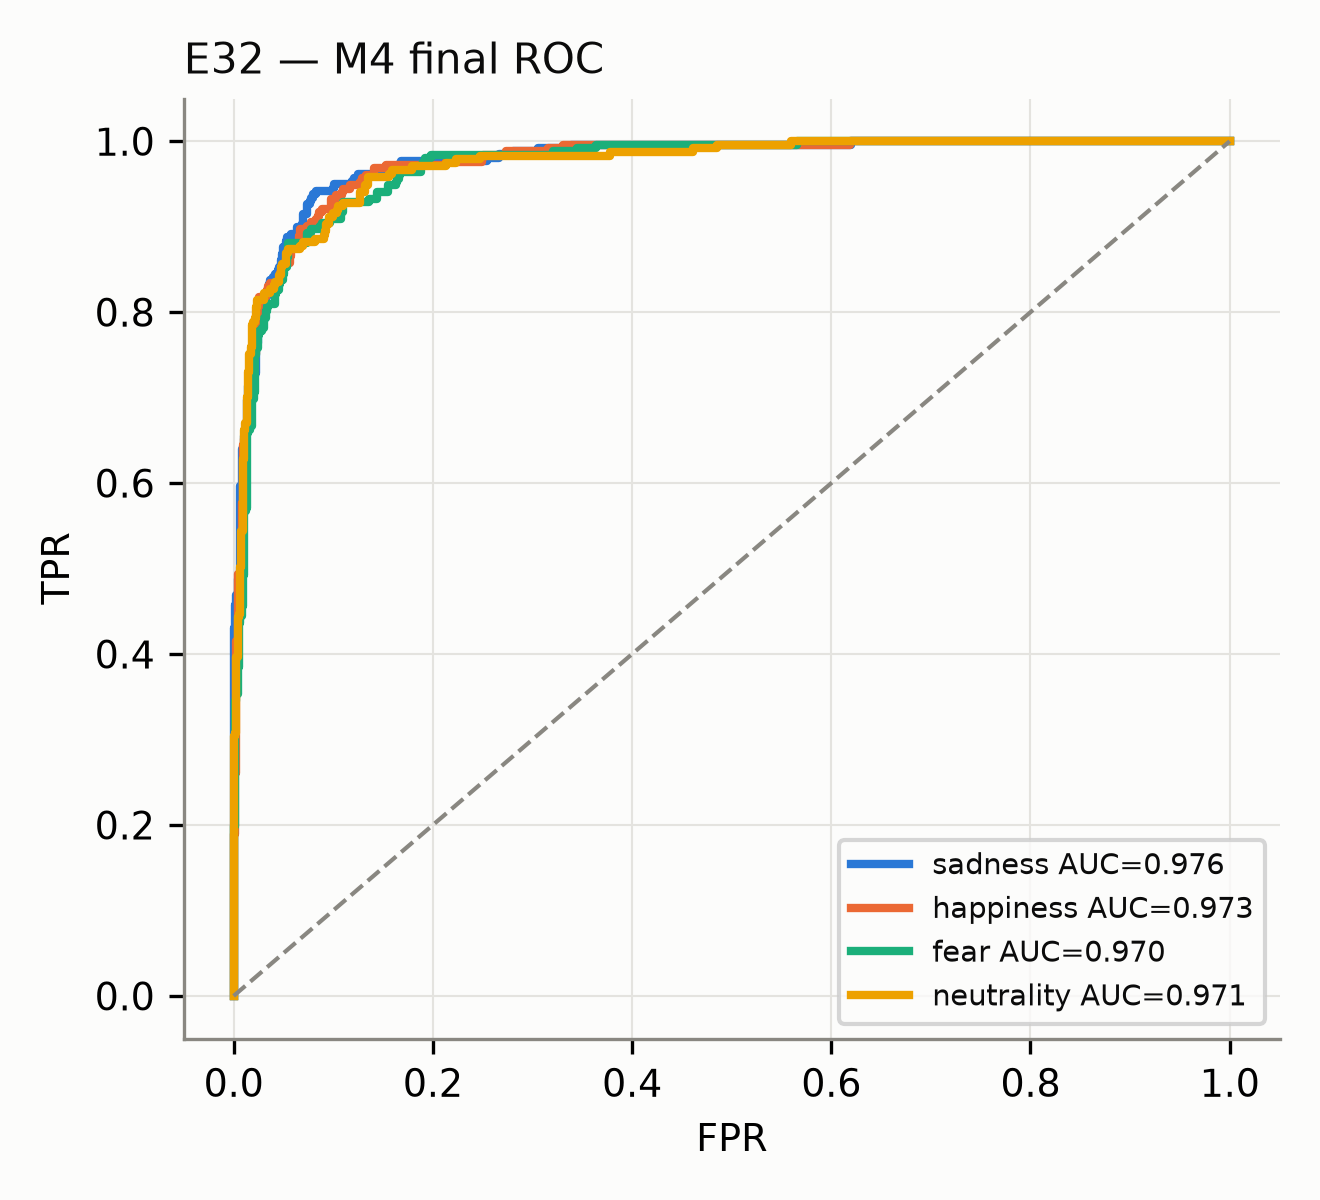
\includegraphics[width=0.55\linewidth]{32_final_roc_curves.png}
\caption{M4 one-versus-rest ROC curves from the same pooled probability file.}
\label{fig:roc}
\end{figure}

\begin{figure}[t]
\centering
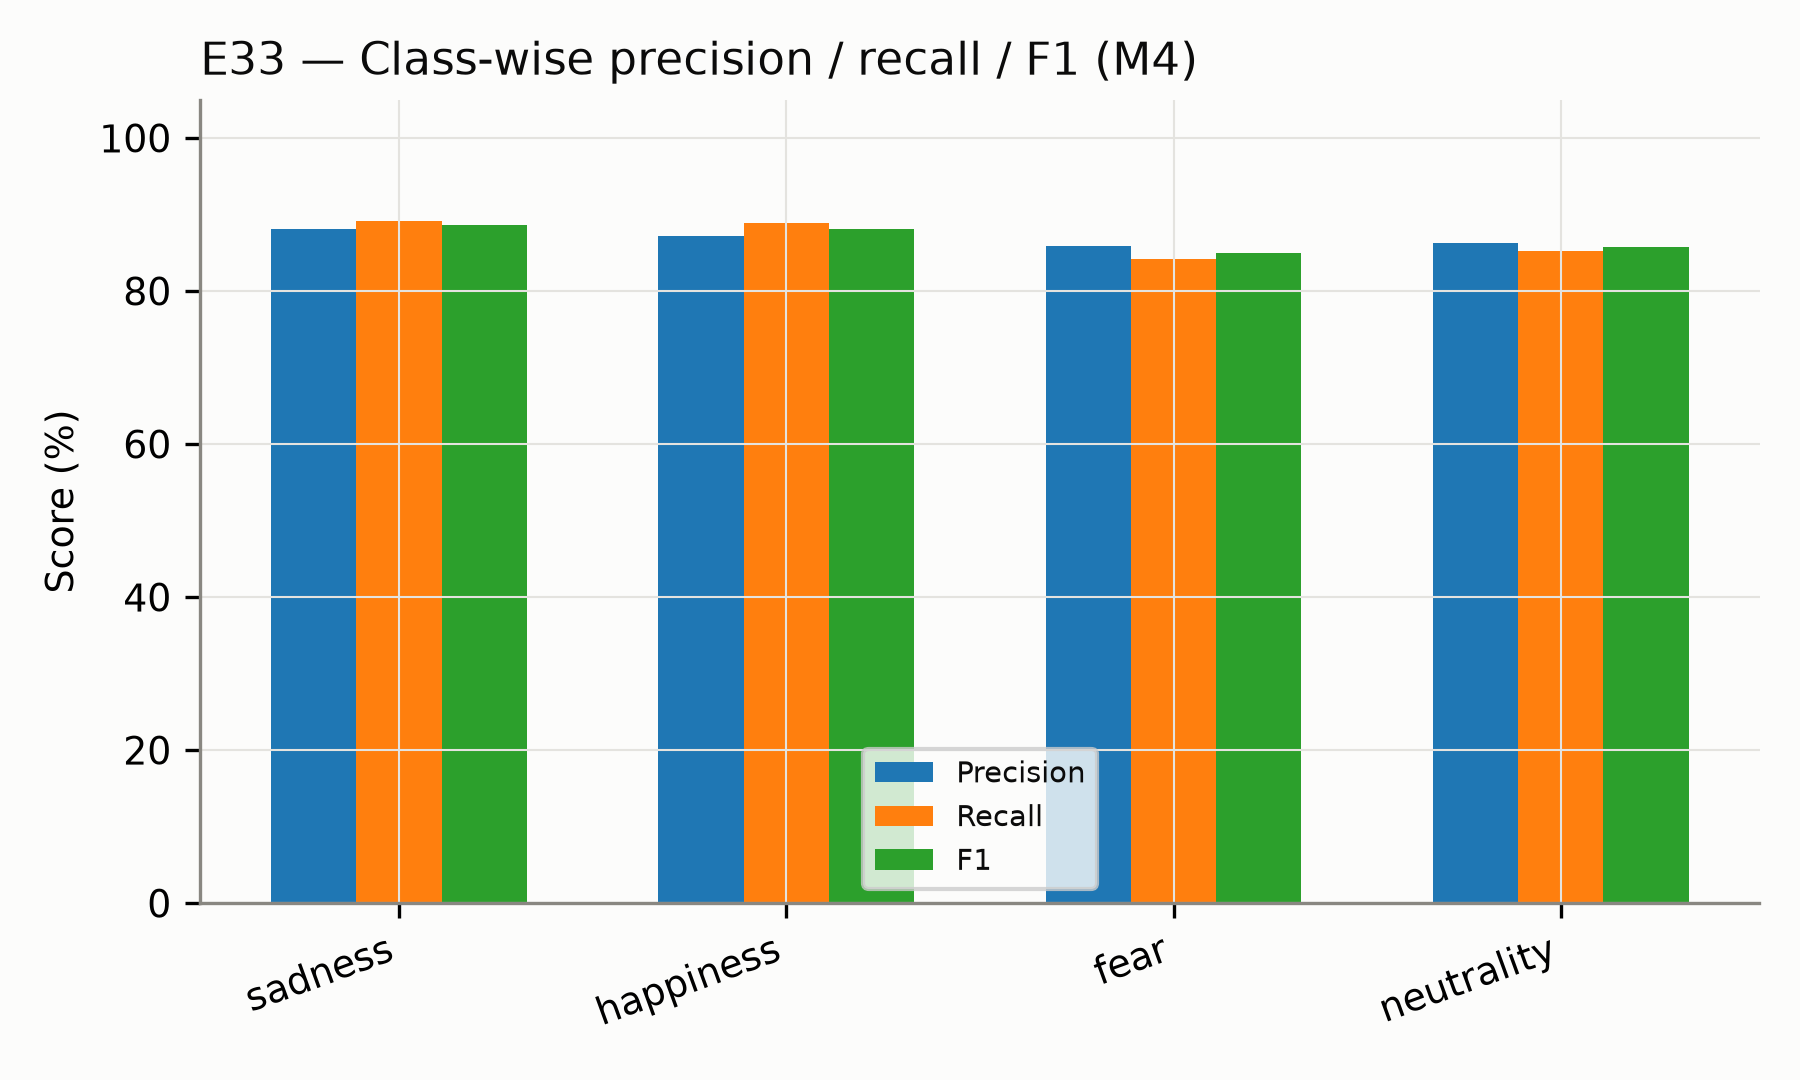
\includegraphics[width=0.7\linewidth]{33_classwise_precision_recall_f1.png}
\caption{Class-wise precision, recall and F1 corresponding to the pooled M4 predictions used for the figure (see text).}
\label{fig:cls}
\end{figure}

\subsection{What the scenario supports}
Continuous weights are not automatically more accurate than a hard gate when the underlying band is weaker (M1 versus M0). Mixing a strong band with a weaker one (M2) can recover accuracy without fusion. Late fusion helps when bands err differently (M3 above every single band on both scales). Adding the adaptive gate on top of fusion (M4 versus M3) is slightly helpful on one scale and slightly harmful on the other. Those statements are properties of the generator, not of the public datasets.

\section{Discussion}
Pupil features respond to luminance and individual baselines \cite{Kret2019,Mathot2018}; a hard threshold on an uncorrected trace can therefore keep the wrong windows. Equation~\eqref{eq:fuzzy} keeps a minimum weight of $0.1$, so weak windows still contribute, which is desirable only when the residual signal is informative. Subject-specific baselines in M2 address a different error---offset---and smoothing addresses isolated spikes. Neither operation changes the EEG rule base.

Fusion \eqref{eq:fuse} can exploit complementary mistakes only when the band posteriors differ. If one band already dominates, learned weights concentrate on that band and the gain over the best single band is modest, which is what Table~\ref{tab:bandsyn} shows for alpha versus M3. Window-selection quality (Table~\ref{tab:gate}) is not the same quantity as emotion accuracy (Table~\ref{tab:synth}). The eye-gate rules in the appendix must not be read as emotion rules.

\section{Limitations and future work}
The M0--M4 numbers in Section~\ref{sec:results} are synthetic. They do not validate the system on SEED-IV or MAHNOB-HCI. The illustrative heads are not trained Sugeno classifiers. DWT bands in code do not match the paper's stated Hertz limits exactly. Several GA rates are unspecified in the paper and are therefore not invented here. Pupil diameter confounds emotion with light and load. A credible next step is subject-independent evaluation on synchronised recordings, with the production FIS--GA path, inner-fold fusion weights, and paired statistical tests \cite{Demsar2006} computed on those predictions only.

\section{Conclusion}
The 2024 hard-gated fuzzy pipeline \cite{FarhadiSedehi2024a} remains the reference method: binary eye gating, per-band entropy features, Sugeno rules and a genetic algorithm, with published alpha-band accuracies of 94.42\% (SEED-IV) and 85.20\% (MAHNOB-HCI). The repository adds a continuous eye gate, an adaptive temporal variant, and late fusion of five band probabilities. A deterministic synthetic scenario shows that these changes are not uniformly beneficial: fuzzy gating of a weaker band underperformed the hard-gated alpha head, while fusion was the most reliable gain, and the full M4 combination beat M3 on only one of the two reference scales. Those outcomes motivate real-data experiments; they do not replace them.

\section*{Abbreviations}
EEG, electroencephalography; FIS, fuzzy inference system; GA, genetic algorithm; mRMR, minimum redundancy maximum relevance; DWT, discrete wavelet transform; AUC, area under the ROC curve; S-FIS, Sugeno FIS.

\section*{Principal notation}
$z(t)$ normalised pupil feature; $\mu_i$ membership; $r_i$ Sugeno gate consequent; $w(t)$ gate weight; $P_b(c)$ band-$b$ probability of class $c$; $w_b$ fusion weight.
